% Chapter 3
\makeatletter
\def\input@path{{../}}
\makeatother
\documentclass[../main.tex]{subfiles}
\begin{document}
\chapter{Characteristics of single particle motion in a Burgers vortex} % Chapter title

\label{ch:single} % For referencing the chapter elsewhere, use \autoref{ch:single}

%----------------------------------------------------------------------------------------
This chapter addresses the dynamics of the system, which is the particle moving in a Burgers vortex, defined by the set of differential equations (Eq.\ref{ch2:eq03a}-\ref{ch2:eq03c} and its dimensional counterpart). The system differs significantly depending on gravity presence. First, with the use of dynamical system formalism, the system is stratified into its orbits and dynamics of these orbits is determined. Second, particular emphasis is placed on describing the characteristic time scales of the motion and their mutual relations. These tasks are performed with the hope of finding a measure of spatial pattern formation efficiencyn in relation to model parametes.\\
It was stated before, that the equation describing particle motion along the vortex axis (Eq. \ref{ch2:eq03c}) is independent from the ones describing motion in 2D space (Eq.\ref{ch2:eq03a}-\ref{ch2:eq03b}). Thus in this chapter they are analysed in separate sections.
 
\section{Motion along the vortex axis}
% In this thesis analytical solution presented in \citep{Karpinska2014} is extended to accound for (...).
Particle motion along the vortex axis is determined by stretching outflow drag and gravity force only. As a consequence, the particle position along axis shows an exponential dependence on time, which is explained below.\\
In this dimension, every particle has one equillibrium point $z_b$, so according to the definition in Sec.\ref{ch2s2} a point in which $\ddot{z}=0,\ \dot{z}=0$. Its dimensional and dimensionless relation to system parameters:
\begin{align}
z^+_b=S_v A^{-1} \cot\theta\\
z_b=z^+_b \delta=\nu^{-1}g \delta^2 \tau_p cos\theta \propto R^2
\label{def:z_b}
\end{align}
Gravity force and stretching can balance only if $z$ is positive, so $z_b>0$. It is a source, so a kind of an unstable equillibrium. Position $z_b$ with respect to vortex core size $\delta$ and particle radius $R$ for cloud-like conditions, is plotted in Fig.\ref{fig:ch3_0}.

\begin{figure*}
\centering
\noindent 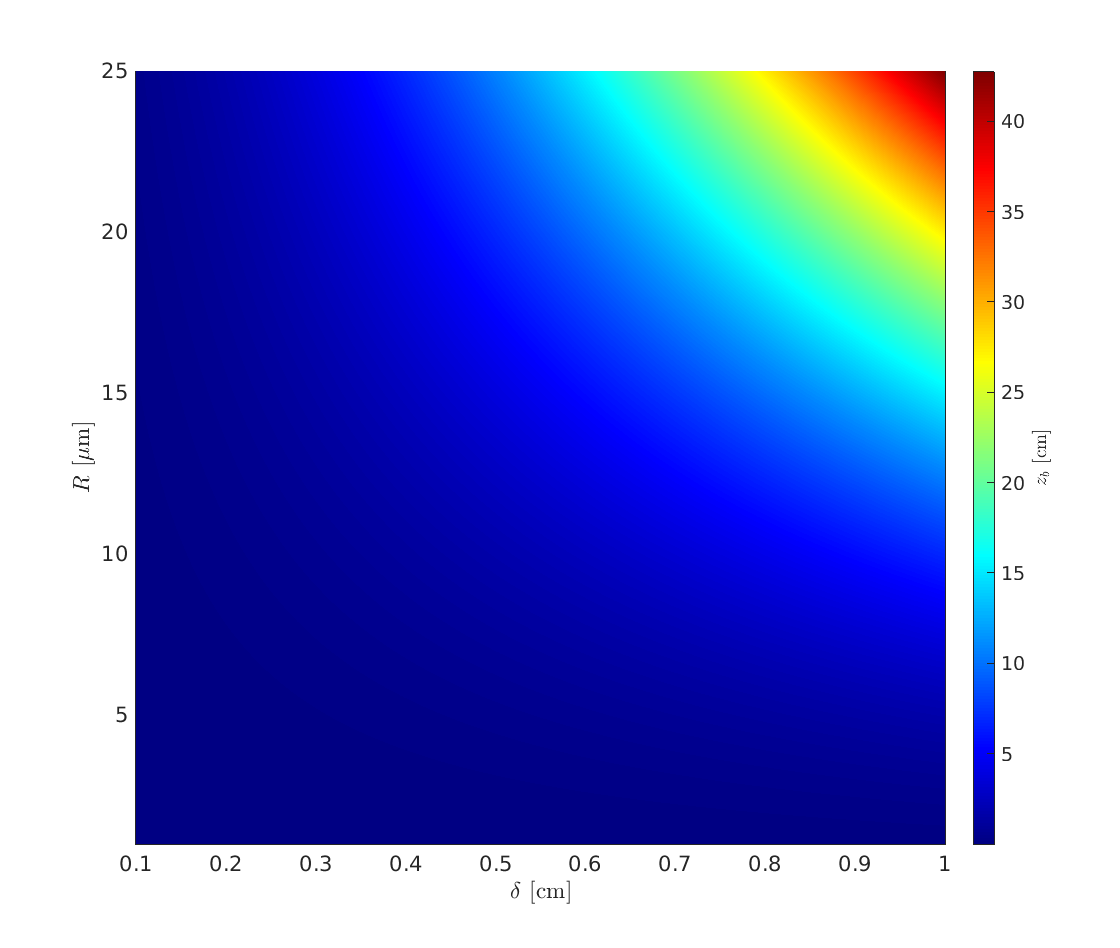
\includegraphics[width=30pc]{gfx/z_b_vs_delta_R.png}
\caption{Equillibrium position $z_b$ versus vortex core size $\delta$ and particle radius $R$. Plot variables' ranges correspond to cloud-like conditions.}
\label{fig:ch3_0}
\end{figure*}

Eq. \ref{ch2:03c} can be integrated with arbitrary constants $C_1$ and $C_2$ leading to the following general solution:
\begin{equation}
z^+(t)=C_1 \exp{\lambda_1 t^+}+C_2 \exp{\lambda_2 t^+}+z^+_b
\label{ch3:eq05}
\end{equation}
so $z^+(t)$ indeed depends exponentially on time.
By setting the initial conditions to $z^+(0)=z^+_0$, $\dot{z}(0)=w_0$ one obtains the following specific solution:
\begin{align}
\frac{z^+(t^+)-z^+_b}{z^+_0-z^+_b}=\frac{1}{\lambda_1-\lambda_2} \left[ \lambda_1 \exp{\lambda_2 t^+}-\lambda_2 \exp{\lambda_1 t^+} + \frac{w^+_0}{z^+_0-z^+_b}\left( \exp{\lambda_1 t^+}- \exp{\lambda_2 t^+}\right)\right] \\
\lambda_{1/2}=\left( \mp \sqrt{1+4 A St}-1\right)/2 St
\label{ch3:eq06}
\end{align}
This equation describes particle motion along the axis, by expressing the evolution of particle distance from equilibrium point with respect to its initial distance from the equilibrium point. In order to give a sense of this solution, it was rewritten using the newly defined dimensionless $k$ parameter:
\begin{equation}
k=(1+4 A St)^{-\frac{1}{2}}=(1+2\tau_p \gamma)^{-\frac{1}{2}}
\end{equation}
where $k \in (0,1)$, and dimensionalized:
\begin{equation}
\frac{z(t)-z_b}{z_0-z_b}=
\left[\frac{1}{2}\left(1-k\right)-k\frac{\tau_p w_0}{z_0-z_b}\right] e^{\frac{-t}{2 \tau_p}(k^{-1}+1)}+
\left[\frac{1}{2}\left(1+k\right)+k\frac{\tau_p w_0}{z_0-z_b} \right] e^{\frac{t}{2 \tau_p}(k^{-1}-1)}.
\label{ch3:eq08}
\end{equation}
One can see that the first term in \ref{ch3:eq08} is leading for small times, especially when the initial velocity is nonzero. In longer times the second term is a leading term.\\
As has already been argued in the introduction, the Burgers vortex is a good approximation for a long-lasting vortex only locally in space and time in turbulent flow. Therefore, the motion of particles in a vortex which has finite size and lifetime should be considered. For this reason further discussion of particle motion along the axis is devoted to the estimation of what is here defined as \emph{exit time} $\tau_{ex}$:\marginpar{exit time} the time at which a particle starting at position $z(t=0)=z_0$, with zero initial velocity $\dot{z}(t=0)=0$, reaches an arbitrary finite domain border $\pm Z$.\\
First, the Eq. \ref{ch3:eq08} for the initial velocity set to zero, $w_0=0$, simplifies to:
\begin{equation}
\frac{z(t)-z_b}{z_0-z_b}=\frac{1}{2}\left(1-k\right) e^{\frac{-t}{2 \tau_p}(k^{-1}+1)}+\frac{1}{2}\left(1+k\right) e^{\frac{t}{\tau_p}(k^{-1}-1)}
\label{ch3:eq11}
\end{equation}
In this case, the direction of motion depends on the relative position of $z_0$ and $z_b$ only. This thesis assumes that particles are significantly smaller then vortex size: $R<<\delta$, and thus $\tau_p \gamma <<1$. In large times $t>>\tau_p$ this assumption allows to approximate Eq.\ref{ch3:eq11} to:
\begin{equation}
\frac{z(t)-z_b}{z_0-z_b}=e^{\frac{t}{\tau_z}}
\label{ch3:eq12}
\end{equation}
where $\tau_z$ is the characteristic time of the motion along vortex axis:
\begin{equation}
\tau_z=\frac{2}{k^{-1}-1} \tau_p=\frac{2}{\sqrt{1+2\tau_p \gamma}-1} \tau_p
\label{ch3:eq09}
\end{equation}
According to small particles assumption, $\tau_z$ can be approximated as well:
\begin{equation}
\tau_z\approx \frac{2 \tau_p}{1+ 2\tau_p \gamma/2 -1}=2\gamma^{-1}=\nu^{-1}\delta^2.
\label{ch3:eq10}
\end{equation}

\begin{figure*}
\centering
\noindent 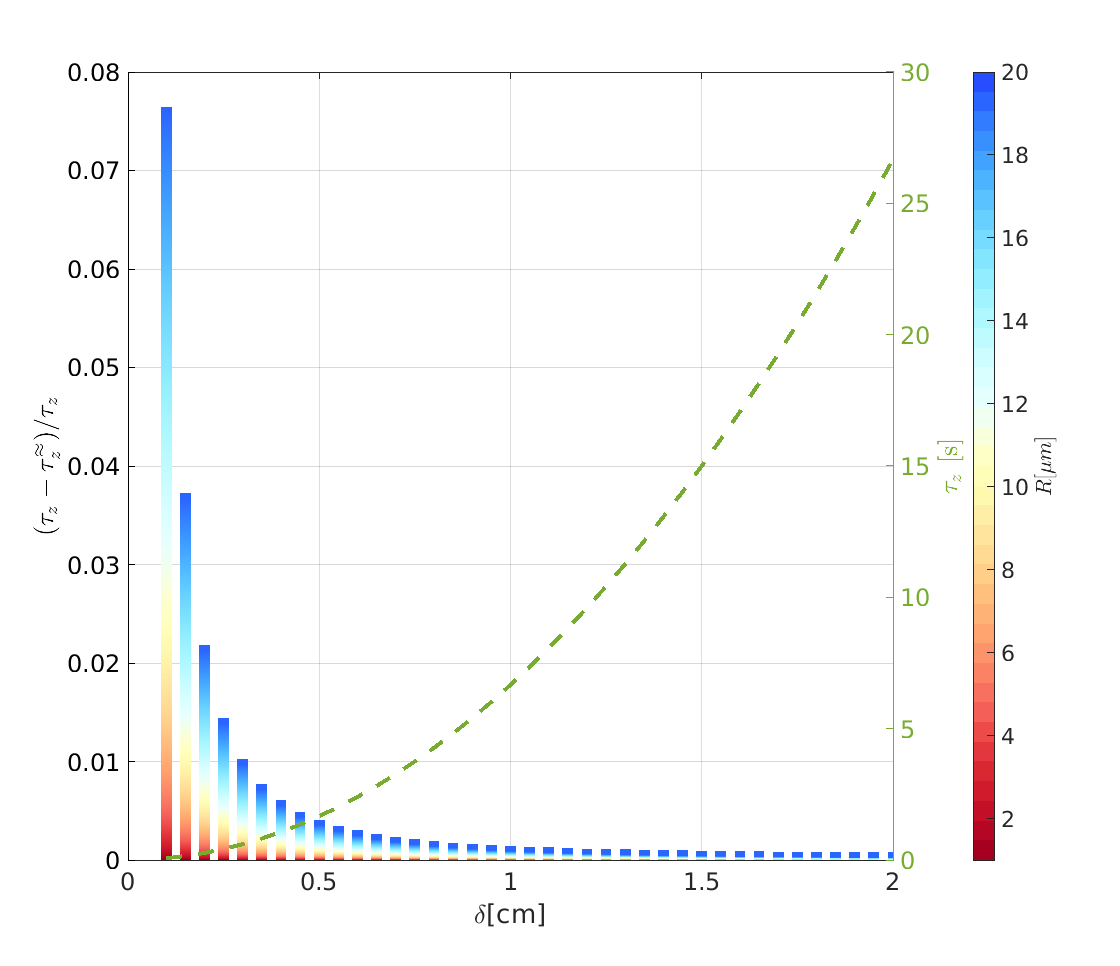
\includegraphics[width=30pc]{gfx/tau_z_error_tau_z_vs_delta.png}
\caption{Characteristic time of the motion along vortex axis $\tau_z$ (green line, right y-axis) versus vortex core size $\delta$ and its relative error (left y-axis, bar chart) versus $\delta$ and particle radius $R$. Colorscale indicates dependence on $R$. Plot variables' ranges correspond to cloud-like conditions.}
\label{fig:ch3_1}
\end{figure*}

Figure \ref{fig:ch3_1} presents $\tau_z$ relative arror (accurate value from Eq.\ref{ch3:eq09} minus approximated value from Eq.\ref{ch3:eq10} divided by the acurate value) with respect to $\delta$ (on X-axis) and $R$ (color). We see that for cloud-like variables' ranges the approximation is fully justified. What is interesting is that the approximated $\tau_z$ does not depend on particle size, so it is the same for all the particles in polydisperse dispersion. It is also easy to notice that in cloud-like conditions particle response time is always significantly smaller then characteristic time of motion along axis $\tau_z>>\tau_p$. For example when the vortex core size $\delta$ is 1~cm, then $\tau_z$ is approximately 6.7~s, and for 0.5cm it is approximately 1.6~s.\\
The simplified equation of motion, Eq.{ch3:eq12}, must be solved in order to estimate the exit time:
\begin{equation}
\frac{sign(z_0-z_b)Z-z_b}{z_0-z_b}=e^{\frac{\tau_{ex}}{\tau_z}}
\label{ch3:eq07}
\end{equation}
so there is:
\begin{equation}
\tau_{ex}=\tau_z \log\left(\frac{sign(z_0-z_b)Z-z_b}{z_0-z_b} \right)
\label{ch3:eq12b}
\end{equation}
The function under the logaritm is denoted as $L(Z,z_0;z_b)$ and further:
\begin{equation}
L(Z,z_0;z_b)=\frac{Z-sign(z_0-z_b)z_b}{|z_0-z_b|}=\frac{Z/z_b-sign(z_0-z_b)}{|z_0/z_b-1|}=
\frac{\overbrace{Z/z_b}^{Z^\ast}-sign(z_0/z_b-1)}{|\underbrace{z_0/z_b}_{z_0^\ast}-1|}.
\label{ch3:eq13}
\end{equation}
Then the estimated exit time:
\begin{align}
\tau_{ex}(Z^\ast,z_0^\ast; \tau_z)\approx \tau_z \log\left(L(Z^\ast,z_0^\ast)\right)\\
L(Z^\ast,z_0^\ast)= \frac{Z^\ast-sign(z_0^\ast-1)}{|z_0^\ast-1|}\\
\label{ch3:eq14}
\end{align}
where $Z^\ast \in (1,\infty), \ z_0^\ast \in [-Z^\ast,1)\cup (1,Z^\ast]$. For $z_0^\ast=1$ (when $z_0=z_b$) the estimation gives $\tau_{ex}=\infty$, so it agrees with the fact, that $z_b$ is an unstable equillibrium point.

\begin{figure*}
\centering
\noindent 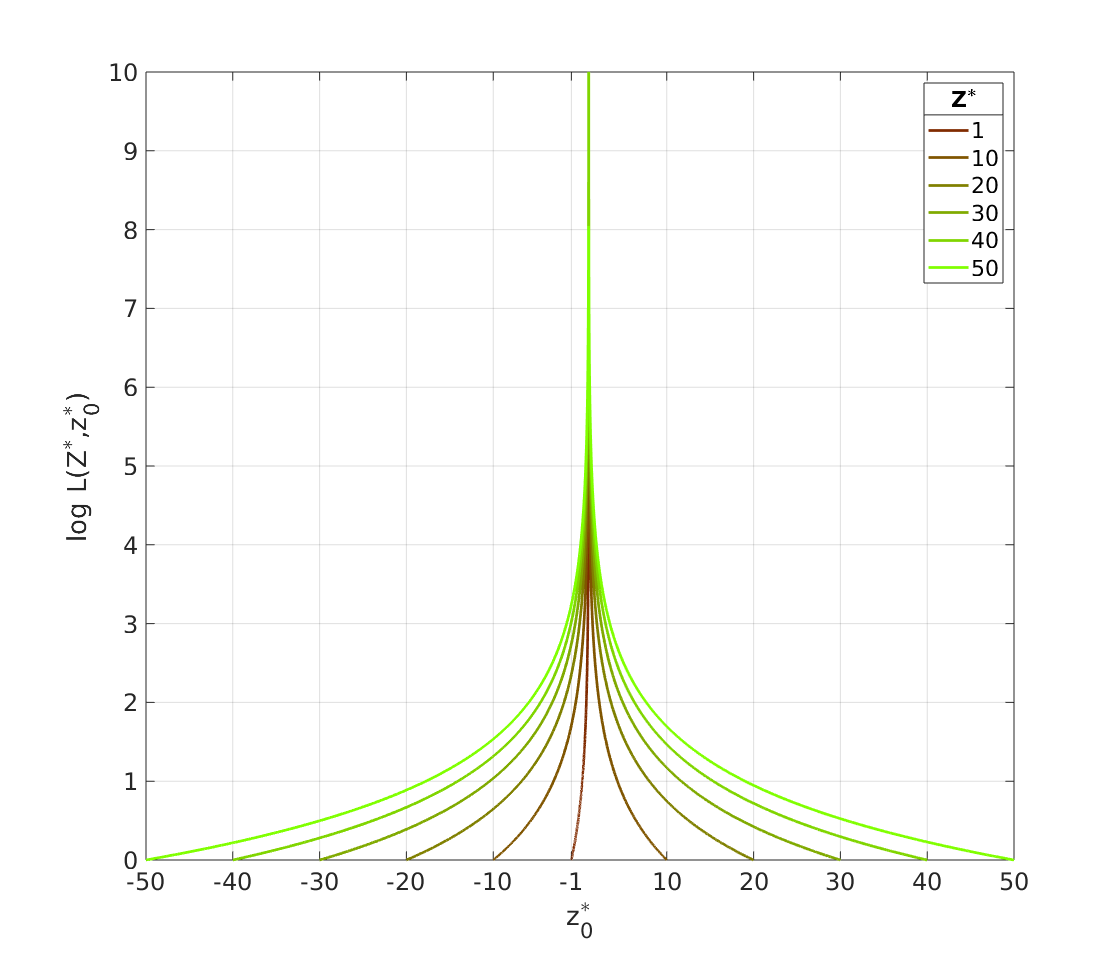
\includegraphics[width=30pc]{gfx/Z_log_factor_plot.png}
\caption{Logarithmic factor $logL$ (in $\tau_{ex}$) vs. $z^*_0$ - ratio of initial position and equillibrium position. Line color is scaled by $Z*$ values which refer to different ratios of vortex half-length and equillibrium position.}
\label{fig:ch3_2}
\end{figure*}

The logarithmic factor in $\tau_{ex}$ is depicted in Fig. \ref{fig:ch3_2}. It depends on domain half-length $Z$ and initial position $z_0$ ratios to $z_b$. It is hard to draw any direct conlusions for single particle exit time on the basis of Fig.\ref{fig:ch3_2} alone. However there is an interesting feature when thinking about the collection of particles in the vortex. Namely, the mean value of logarithmic factor over $z_0^\ast$ (over all initial positions) equals one for every $Z^\ast$ (for every vortex half-length):
\begin{equation}
\langle log\ L(Z^\ast,z_0^\ast)\rangle_{z_0^\ast}=\frac{1}{2 Z^\ast}\int_{-Z^\ast}^{Z^\ast}log\ L(Z^\ast,z_0^\ast)dz_0^\ast=1
\label{ch3:eq15}
\end{equation}
This means that independently of vortex length, when dealing with uniformly distributed set of particles, the logarithmic factor does not have influence on mean exit time.

\section{Motion in the plane perpendicular to vortex axis}

The trajectories determined in 2D space by Eq.\ref{ch2:eq03a}-\ref{ch2:eq03c} have several different attractors. The exact choice depends on the system parameters. Presence of gravity force distinguishes two basic cases. There are presented below.
%The analysis of single droplet motion in projection on a plane $(r,\varphi)$ perpendicular to the vortex axis was conducted by \citet{Marcu1995} and is summarized below.

\subsection{Without gravity (vertical vortex)}
The system without gravity force in 2D space is equal to the system in which gravity is parallel to the vortex axis ($\theta=0$). It comes down to the fact that sedimentation parameter $S_v$ is zero. In this case the nondimensional equations of motion are:
\begin{equation}
\left\{\begin{array}{l}
\ddot{r^+}-r^+\dot{\varphi^+}^2=-St^{-1}\left(A r^++\dot{r^+}\right) \\
2\dot{r^+}\dot{\varphi^+}+r^+\ddot{\varphi^+}=St^{-1}\left(\frac{1}{2 \pi r^+}(1-e^{-\frac{r^{+ 2}}{2}})-r^+\dot{\varphi^+}\right)\\
\end{array}.\right.
\label{ch3:eq16}
\end{equation}
and the system posses axial symmetry. This set of equations depends on two parameters only: $St/A$ and $St$. The attractors: an equilibrium point positioned on the vortex axis $r^+=0$ or a circular orbit of radius $r^+_{orb}$ (defined later), inherit the axial symmetry. The system changes according to Hopf bifurcation scheme. Lets put $\alpha=16 \pi^2-St/A$ as a bifurcation parameter. This translates to the fact, that if:
\begin{equation}
St \leq St_{cr}(A) \equiv 16 \pi^2 A,
\label{ch3:eq17}
\end{equation}
the only attractor, the equilibrium point at the axis, is a stable focus ($\alpha \leq 0$). In the opposite case $St > St_{cr}$, the equilibrium point is an unstable focus, accompanied by a stable periodic circular orbit ($\alpha>0$). Particle trajectories around such attractors are presented schematically in Fig. \autoref{fig:ch2_04}. Having established the existence of attractors, their impact on particle kinematics is studied.\\

\subsubsection{Stable periodic orbit}

The first type of trajectory that is analysed is the particle moving on stable periodic orbit. The radius of the periodic orbit, denoted as $r^+_{orb}$, satisfies the equation:
\begin{equation}
 \left[1-\exp\left( -r^{+ 2}/2 \right) \right]/2 \pi r^{+ 2}=\sqrt{A/St}, 
\label{ch3:eq18}
\end{equation}
which depends uniquely on $St/A$. Fig. \ref{fig:ch3_3} presents numerical solution of this equation. For ease of reference, X-axis shows $r^{+ 2}_{orb}$ and Y-axis shows $\sqrt{St/A}$. Two asymptotic limits are included as well. For small orbit radius, $r^+_{orb}<<1$, it is possible to approximate left-side of Eq.\ref{ch3:eq18} by developing Taylor series around zero and get:
\begin{equation}
 \left[1-\exp\left( -r^{+ 2}/2 \right) \right]/2 \pi r^{+ 2}\approx \left(\frac{1}{2}-\frac{r^{+ 2}}{8}+O(r^{+ 4})\right)/2 \pi
\label{ch3:eq18a}
\end{equation}
which then gives the relation
\begin{equation}
r^{+ 2} \sim - 16 \pi \sqrt{A/St}+4
\label{ch3:eq18aa}
\end{equation}
shown in Fig.\ref{fig:ch3_3} by curved dashed blue line. On the other side, in the limit of large orbit radius there is:
\begin{equation}
\left[1-\exp\left( -r^{+ 2}/2 \right) \right]/2 \pi r^{+ 2}\approx \left(r^{+ -2}+O(r^{+ -4})\right) /2 \pi
\label{ch3:eq18b}
\end{equation}
which leads to the asymptotic:
\begin{equation}
r^{+ 2}_{orb} \sim \frac{1}{2\pi} \sqrt{\frac{St}{A}}
\label{ch3:eq18c}
\end{equation}
shown in Fig.\ref{fig:ch3_3} as straight dashed blue line.

\begin{figure*}
\centering
\noindent 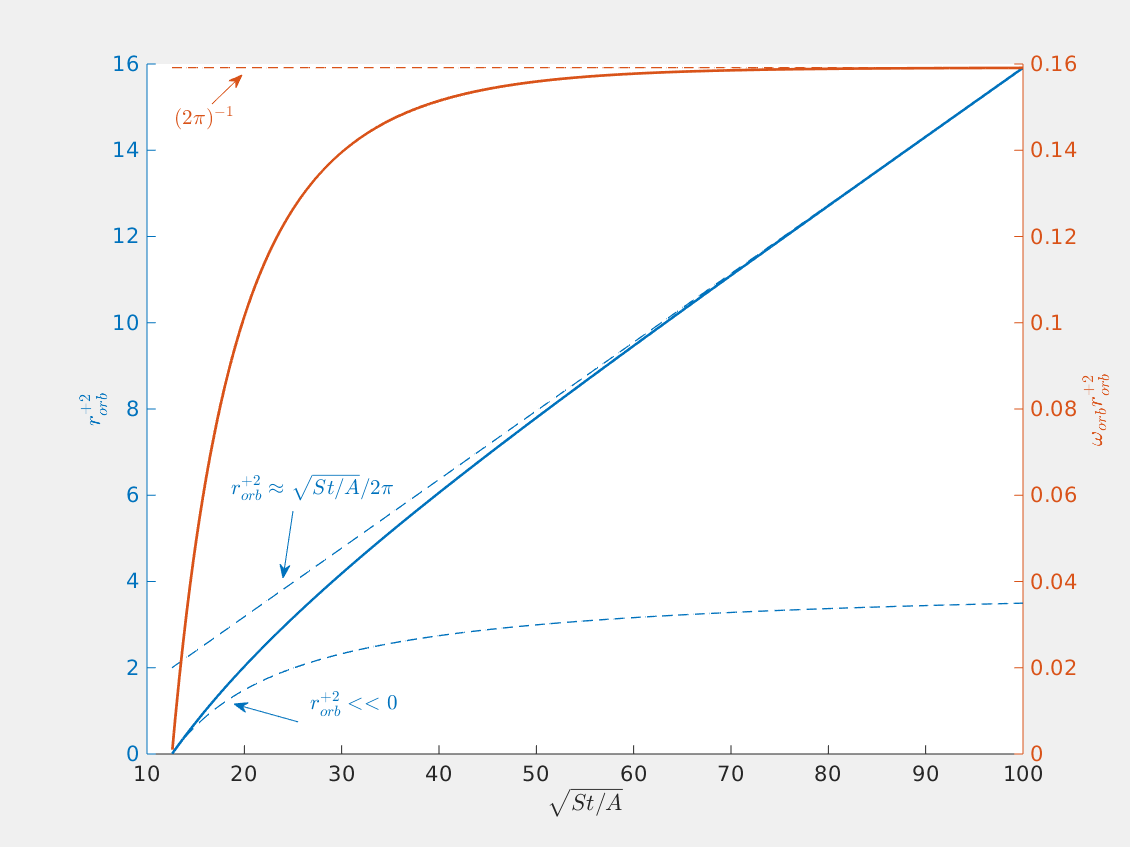
\includegraphics[width=30pc]{gfx/r0_2_sqrt_St_A_omega_r0_2.png}
\caption{Particle stable periodic orbit radius $r^+_{orb}$ square (left y-axis) and orbit nondimensional angular momentum (right y-axis) with respect to parameter $\sqrt{St/A}$. Dashed lines represent asymptotic relations.}
\label{fig:ch3_3}
\end{figure*}

The second conclusion based on the solution to equation \ref{ch3:eq18} is that nondimensional angular velocity at circular periodic orbit is: $\omega^{+}_{orb}=\sqrt{A/St}$, or in other words, particle rotation time $\tau^+_{orb}=\sqrt{St/A}$. What is interesting, particle angular momentum $\omega^{+} r^{+ 2}$ on circular orbit (orange line plot in Fig. \ref{fig:ch3_3}, right Y-axis) in large radius limit is approximately constant in time and independent of particle size, equal to $(2 \pi)^{-1}$. \\
$\sqrt{St/A}$ solely determines orbit stratification in 2D space in no-gravity case and the circular periodic orbit dynamics. It is then important to investigate its connection to dimensional system parameters:
\begin{equation}
\sqrt{\frac{St}{A}}=\sqrt{\frac{2\rho_p}{9 \rho_a}} \frac{R}{A \delta} 
\label{ch3:eq19_0}
\end{equation}
Periodic orbit (non)existence condition from Eq.\ref{ch3:eq17} is reformulated to:
\begin{equation}
R \geq R_{cr}(A,\delta) \equiv 4 \pi \sqrt{\frac{9\rho_a}{2\rho_p}}\delta A \approx 0.84 \delta A,
\label{ch3:eq19}
\end{equation}
or alternatively:
\begin{equation}
A \leq A_{max}(R,\delta)\equiv \sqrt{\frac{2\rho_p}{9\rho_a}}\  \frac{R}{4 \pi \delta}\approx 1.2 \frac{R}{\delta}
\label{ch3:eq19a}
\end{equation}
so the maximal (critical) strain parameter value $A_{max}$ ($A_{cr}$ is designated to another bifurcation process here) in cloud-like conditions is of the order of the droplet radius to vortex radius ratio.
Dimensional periodic orbit is $r_{orb}=r^+_{orb} \delta$, so the solution obviously depends on $\sqrt{St/A}$ parameter only and then is scaled by vortex core size $\delta$.

 The numerical solution presented in Fig.\ref{fig:ch3_3} is now shown in the Fig. \ref{fig:ch3_3a} in dimensional form, where vortex core size is chosen arbitrarily: $\delta=0.5~cm$. In this parameters' range, the particle orbit radius is of the order of vortex core size. One can see, that in the large orbit limit, from Eq.\ref {ch3:eq18c} there is:
\begin{equation}
r_{orb}\propto \sqrt{R \delta A^{-1}}
\label{ch3:eq19b}
\end{equation}
Figure \ref{fig:ch3_30} shows the results of $r_{orb}$ calculation in a different view. It illustrates the contour plots for selected orbit radii (0.5~cm ,1.5~cm, 3~cm). Overlapping (blue on a top, then pink and green) colored surfaces match subspaces of stable periodic orbit existence.

\begin{figure*}
\centering
\noindent 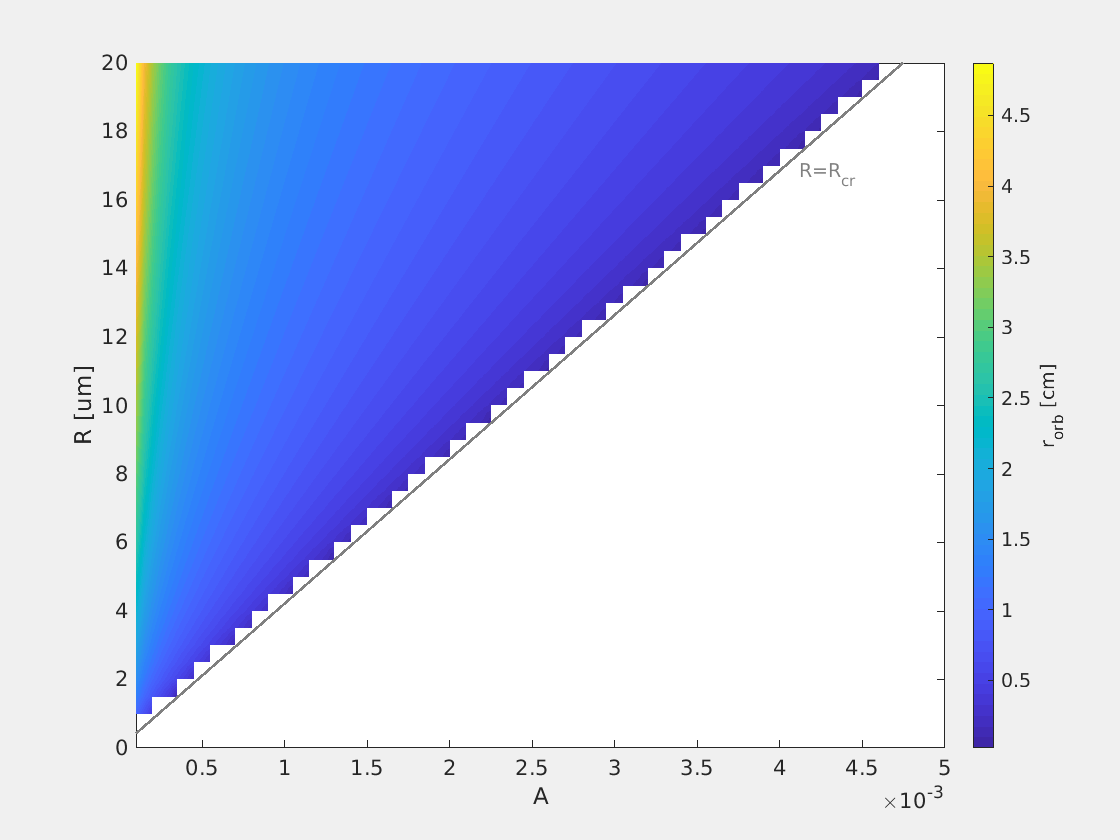
\includegraphics[width=30pc]{gfx/orbit_vs_R_A_delta05cm.png}
\caption{Particle stable orbit radius $r_{orb}$ dependence on  particle radius $R$ and vortex strain parameter $A$ for cloud-like parameter ranges and vortex core size $\delta=0.5~cm$. Black line represents critical parameter value as for stable orbit existence.}
\label{fig:ch3_3a}
\end{figure*}


\begin{figure*}
\centering
\noindent 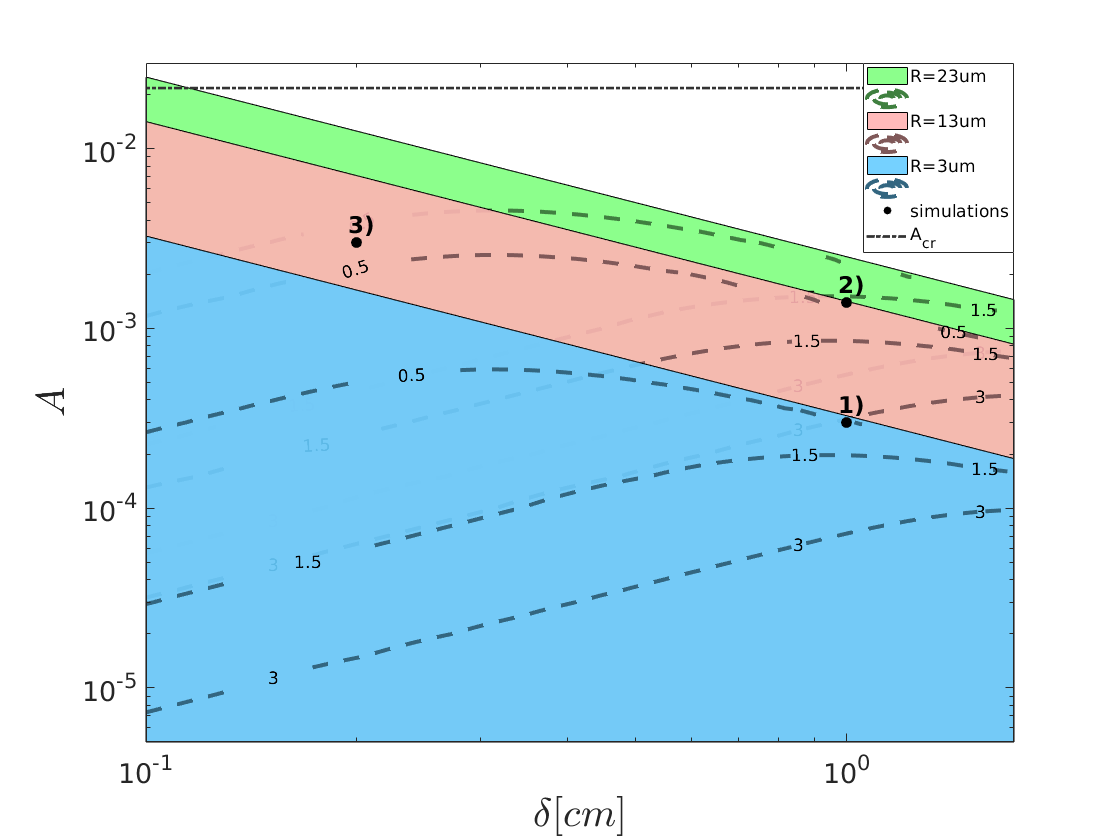
\includegraphics[width=30pc]{gfx/fig05.png}
\caption{Contour plot of stable periodic orbit radius for droplets of radii $R=3,13,23 \ \mu m$ for cloud-like parameter ranges of $\delta$ and $A$. Overlapping (blue on a top, then pink and green) colored surfaces match subspaces in which stable periodic 2D orbit exist for droplet radius given by its colour. Dashed lines are contour plots for $r_{orb}$ equal to 0.5~cm ,1.5~cm, 3~cm. Black points represent simulation parameters sets (refered to in ???).}
\label{fig:ch3_30}
\end{figure*}

It is interesting to notice that the dimensional angular velocity $\omega_{orb}$ is independent of $A$. It is in fact inversely proportional to particle radius $R$ and vortex core size $\delta$:
\begin{equation}
\omega_{orb}=\sqrt{A/St} \tau_f^{-1}=\nu \sqrt{9 \rho_a /2 \rho_p} (R \delta)^{-1} \propto (R \delta)^{-1}.
\label{ch3:eq20}
\end{equation}
Angular velocity on periodic orbit does not depend on $A$, but its existence does. Fig.\ref{fig:ch3_3b} presents cloud-like values of angular velocity $\omega_{orb}$. The existence condition is presented in Fig.\ref{fig:ch3_3b} by $R=R_{cr}(A)$ plots. For a given $A$ periodic orbits exist in  $R>R_{cr}(A)$ area.

\begin{figure*}
\centering
\noindent 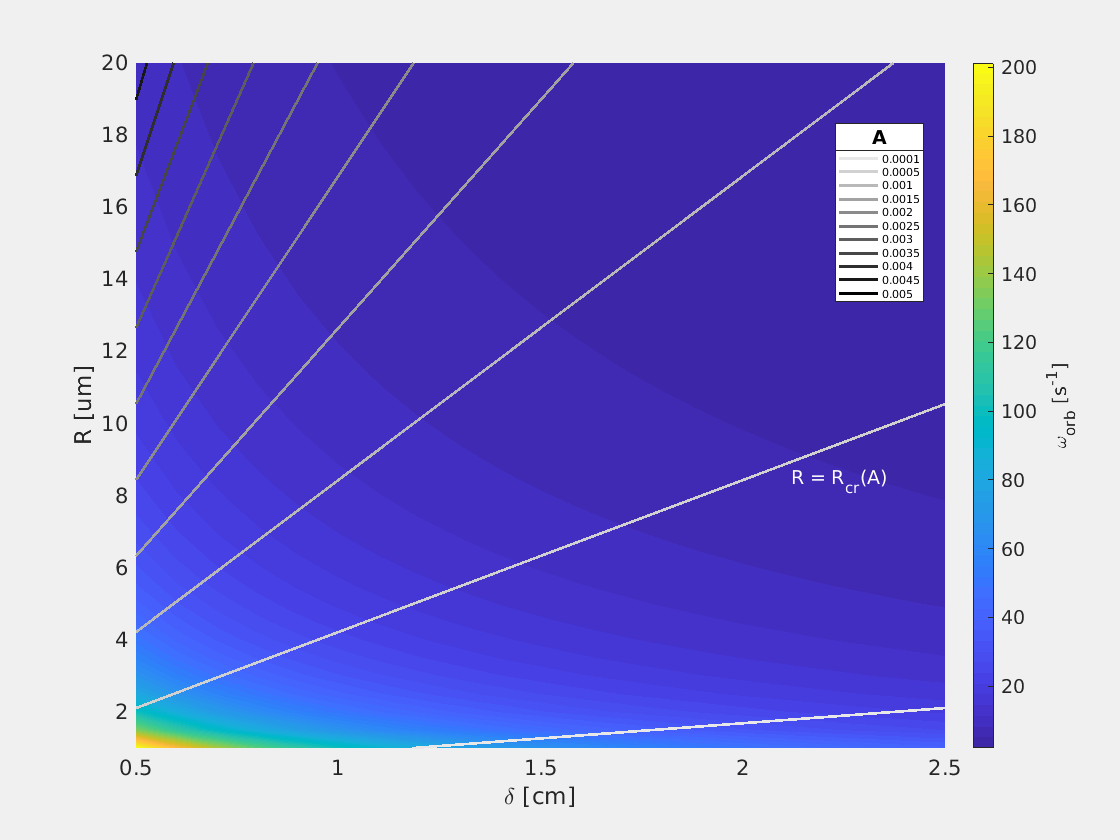
\includegraphics[width=30pc]{gfx/orbit_vel_vs_R_and_delta.png}
\caption{Particle stable orbit angular velocity $\omega_{orb}$ dependence on particle radius $R$ and vortex core radius $\delta$ for cloud-like parameter ranges.}
\label{fig:ch3_3b}
\end{figure*}

Particle rotation time being an inverse of angular velocity is proportional to vortex core radius and particle radius:
\begin{equation}
\tau_{orb}=\sqrt{2 \tau_p \gamma^{-1}} \propto R \delta.
\label{ch3:eq21}
\end{equation}

The previously established assumption of small particles  i.e. $\tau_p<<\gamma^{-1}$ leads to the conclusion that $\tau_{orb}<<\gamma^{-1}$ as well. More on the timescales of motion can be found later in the text.\\
Having identified system attractors and their basic features, their realistic impact on particle kinematic is studied. The probability that a particle founds itself in phase space exactly in the equilibrium point or on periodic orbit is low. More probable is that it is positioned somewhere else and is pulled towards its attractor/s. That fact is the motivation for the detailed study of particles approaching their attractors conducted below.\\

\subsubsection{Stable focus or stable periodic orbit attraction}
I analyze the scales of motion and features of the particle trajectory starting at arbitrary position and approaching its attractor (stable focus at the axis or circular orbit). For the sake of simplicity, the starting radial positions selected for analysis are the only spatial scales distinguished in the equations. That means: the position at the axis $r^+(0)=0$ and at $r^+(0)=r_s$. The motion of a particle defined in this way is called here a "docking process".\marginpar{docking process} Time at which the docking process occures is consequently called docking time and noted $t^+_{doc}$. In short, for the purposes of further analysis, I distinguish two types of processes:
\begin{itemize}
\item in-orbit docking: $r^+(0)=0$, $\dot{r^+}(0)=u_r^+(0)$, particle is attracted by its periodic orbit $r^+_{orb}$
\item axis docking: $r^+(0)=r_s$, $\dot{r^+}(0)=u_r^+(r_s)$ particle is attracted by a point on vortex axis $r^+=0$.
\end{itemize}
Due to the fact, that the particle approaches its destined radial position asymptotically, numerical simulation of the docking process was defined between points in the phase space indicated in the Table \ref{tab:ch3_1}.

\begin{table}
\small
\tabcolsep=0.2cm
\centering
\caption{Initial ($t^+=0$) and final ($t^+=t^+_{doc}$) particle state in numerical simulations of docking processes. $\sigma$ is an arbitrary small parameter.}
\centering
\begin{tabular}{|l||c|c|c|}
\hline 
docking& $r^+(0)$ & $\dot{r^+}(0)$ & $r^+(t^+_{doc})$\\
\hline \hline
in-orbit & $\sigma$ & $u^+_r(\sigma)$ & $r^+_{orb}-\sigma$\\
\hline
axis & $r_s-\sigma$ & $u_r^+(r_s-\sigma)$ & $\sigma$\\
\hline
\end{tabular}
\label{tab:ch3_1}
\end{table}

The choice of small $\sigma$ parameter will be elaborated on later.\\

\begin{figure*}
\centering
\noindent 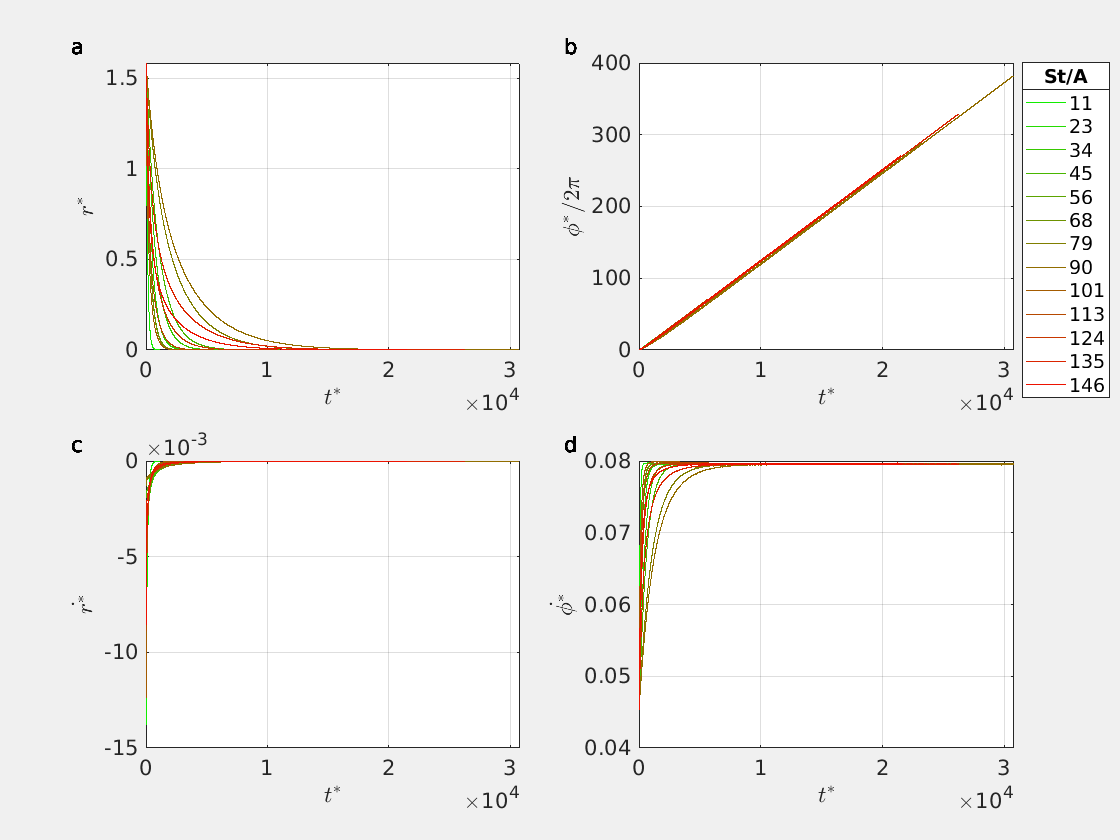
\includegraphics[width=30pc]{gfx/point_docking_vel_traj_in_time_noscal.png}
\caption{Tracking of a particle while docking on axis, for  $\sigma=10^{-4}$. Line color corresponds to $St/A$ value, line color intensity to different $St$ and $A$ representations. Upper panel- radial coordinate, middle panel - radial velocity, lower panel - angular velocity.}
\label{fig:ch3_42}
\end{figure*}

\begin{figure*}
\centering
\noindent 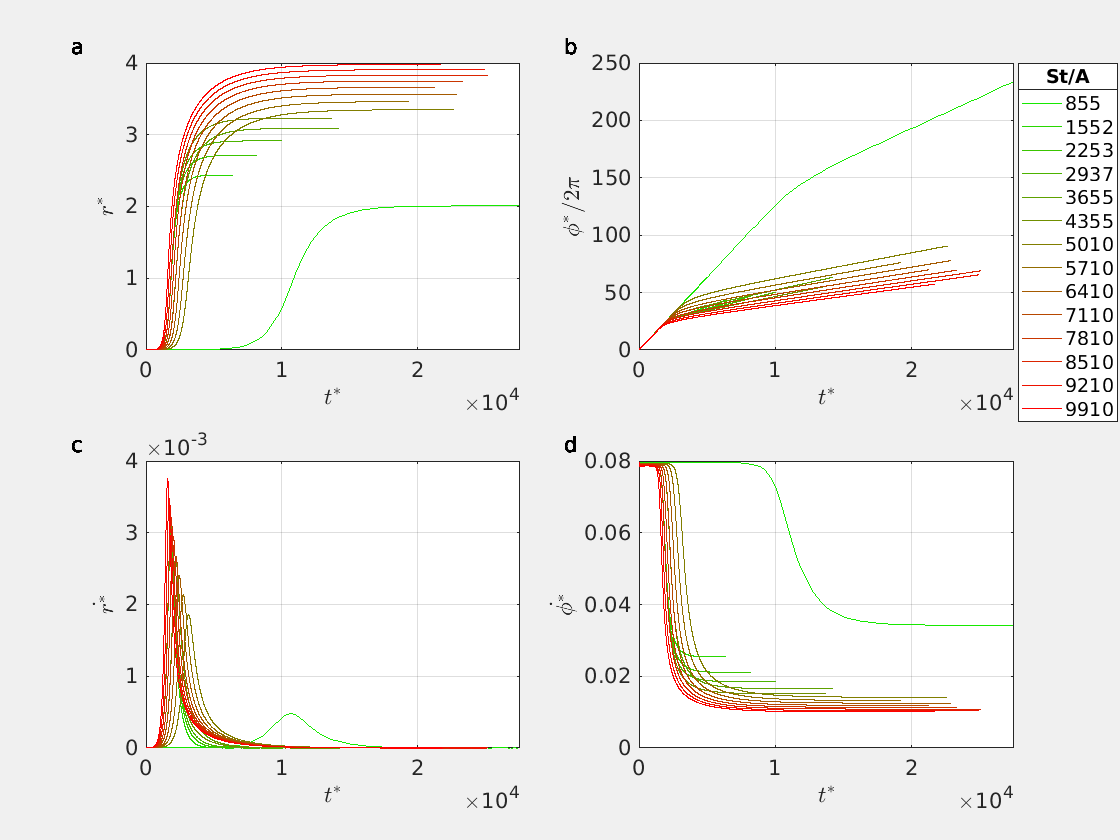
\includegraphics[width=30pc]{gfx/orbit_docking_vel_traj_in_time_noscal.png}
\caption{Tracking of a particle while docking in orbit, for $\sigma=10^{-4}$. Line color corresponds to $St/A$ value, line color intensity to different $St$ and $A$ representations. Upper panel- radial coordinate, middle panel - radial velocity, lower panel - angular velocity.}
\label{fig:ch3_41}
\end{figure*}

Figure~\ref{fig:ch3_42} and Fig.~\ref{fig:ch3_41} show tracking particles wich undergoes docking process, on axis and in-orbit respectively. Three panels show radial position, radial velocity and angular velocity of particles. Each line represents a particle with different $St$ and $A$ parameters. $St$ range was chosen to be $St \in (0,1)$ and $A$ range was adjusted in each case. Line color corresponds to $St/A$ value, line color intensity to different $St$ and $A$ representations of the same $St/A$ value. From Fig.~\ref{fig:ch3_42} it is hard to see any rule on parameter dependence. All the particles tend to have the same angular velocity when they dock on the axis, the radial velocity towards the axis dimnish in time in a kind of exponential manner. The ratio at which it happens depends on both $St$ and $A$, the same is for $t^+_{doc}$. In Fig.~\ref{fig:ch3_42} one can notice, that particles has the same angular velocity at the start and it decreases to a value determined by $St/A$ only. The same time the radial velocity rises and falls again to zero almost symmetrically in time, when the particle reaches its orbit at $r^+_{orb}$. 

\begin{figure*}
\centering
\noindent 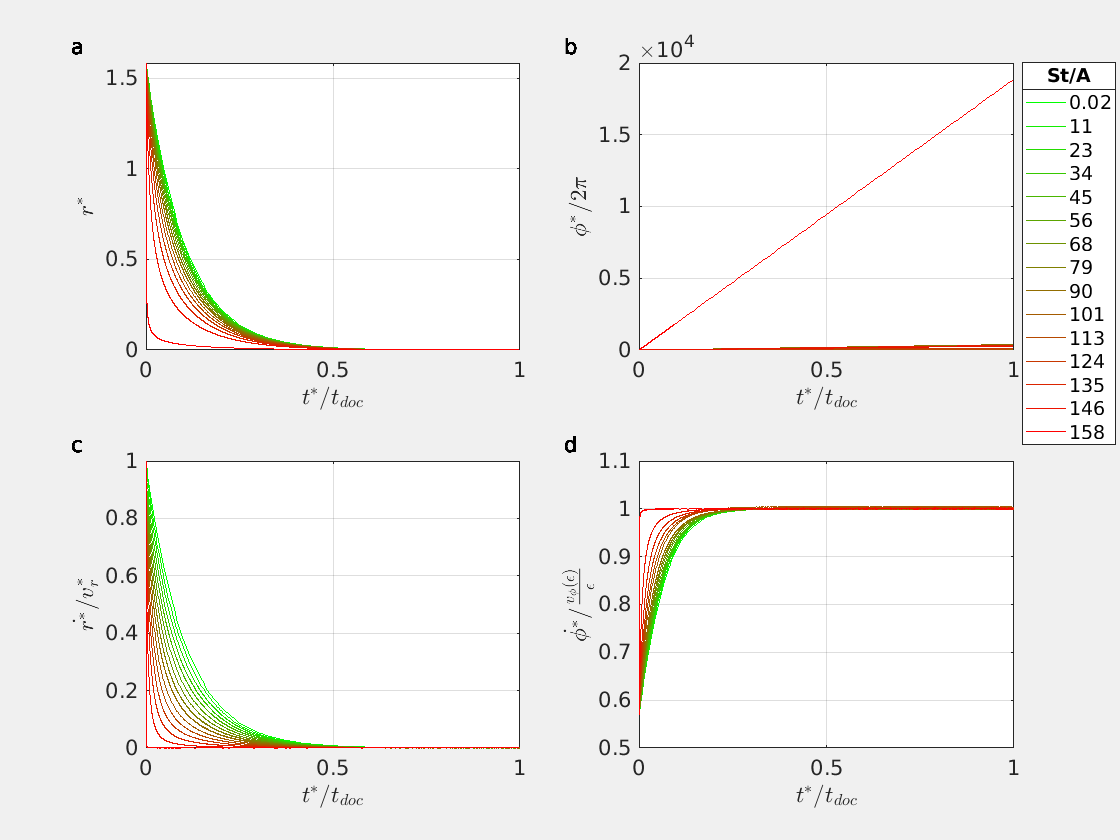
\includegraphics[width=30pc]{gfx/point_docking_vel_traj_in_time_scal.png}
\caption{Same as in Fig. \ref{fig:ch3_42}, but X-axis is scaled separately for each trajectory by a docking time. On Y-axes, the radial velocity is scaled by the fluid velocity at the starting point $u_r(r_s)$, angular velocity is scaled by the fluid angular velocity at the final position $\sigma$, so $u_{\varphi}(\sigma)/\sigma$.}
\label{fig:ch3_44}
\end{figure*}

\begin{figure*}
\centering
\noindent 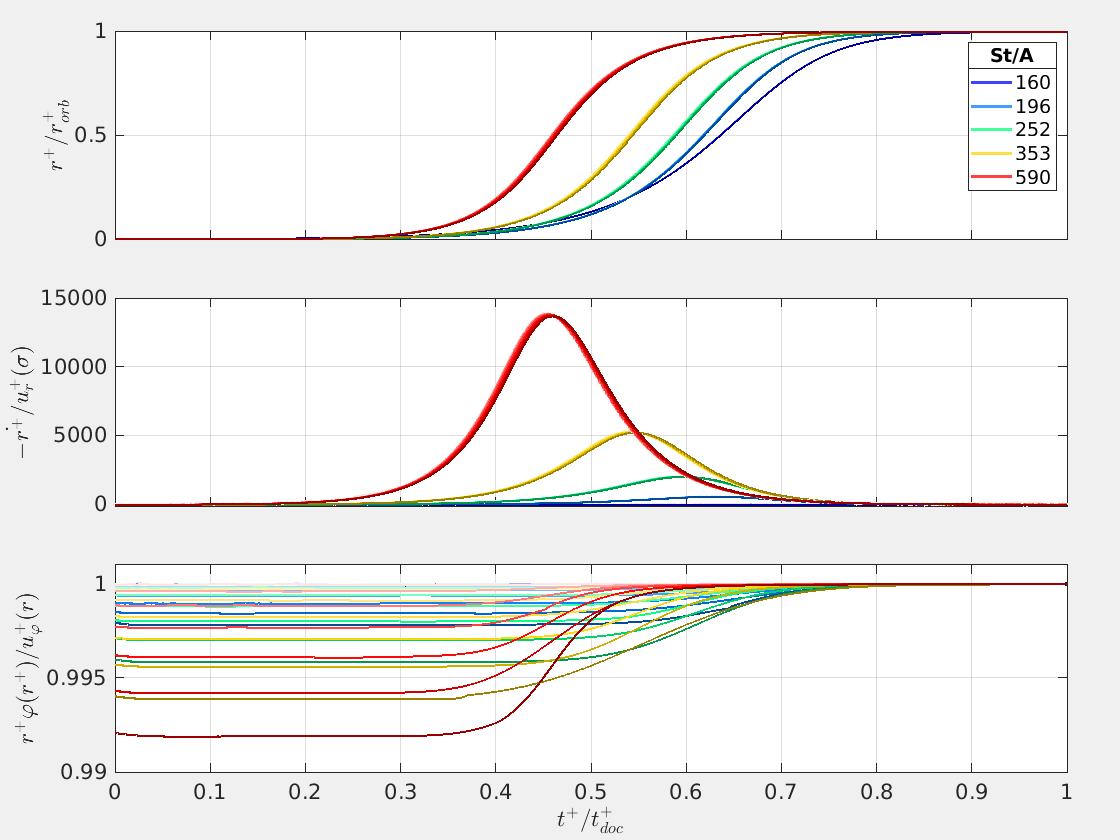
\includegraphics[width=30pc]{gfx/orbit_docking_vel_traj_in_time_scal.png}
\caption{Same as in Fig. \ref{fig:ch3_41}, but X-axis is scaled separately for each trajectory by docking time. On Y-axes, radial position is scaled by circular orbit radius, radial velocity is scaled by the opposite of fluid velocity at the starting point $-u_r(\sigma)$, angular velocity is scaled by the particle angular velocity at the circular orbit $\omega^+_{orb}$.}
\label{fig:ch3_43}
\end{figure*}

Figure~\ref{fig:ch3_44} and Fig.~\ref{fig:ch3_43} represent the same data, but rescaled. X-axis is scaled separately for each trajectory by docking time. In Fig.~\ref{fig:ch3_44}, on Y-axes, the radial velocity is scaled by the fluid velocity at the starting point $u_r(r_s)$, angular velocity is scaled by the fluid angular velocity at the final position $\sigma$, so $u_{\varphi}(\sigma)/\sigma$. In Fig.~\ref{fig:ch3_43},
on Y-axes, radial position is scaled by circular orbit radius, radial velocity is scaled by the opposite of fluid velocity at the starting point $-u_r(\sigma)$, angular velocity is scaled by the particle angular velocity at the circular orbit $\omega^+_{orb}$. By doing so, one can obtain trajectories that depend almost only on $St/A$ parameter - lines of the same color, but different intensity, converge. The greatest difference is seen in particle angular velocity response to fluid, which is caused by different $St$. Fig.\ref{fig:ch3_43} reveals that when the particle is docking in-orbit, it first follows the fluid motion around the axis, with radial velocity close to zero. With rotational velocity, the centrifugal force starts acting on it and causes a rapid increase in radial speed in the direction away from the vortex axis. Increasing distance from the axis in turn results in a steep decrease of the angular velocity, and further the decrease of the radial velocity. Then the particle approaches its periodic orbit: radial velocity goes to zero, rotational velocity goes to $\omega_{orb}$. The rate of these changes depends on the parameters of the model in a complex way. The attempt to find the approximate dependence is conducted below.\\
There is strong time correlation between radial and angular velocity change. In fact when one looks closer at the angular velocity at the particle, it is possible to notice that it depends the most on the radial position of the particle. Figure \ref{fig:ch3_450} presents particle angular velocity in the docking processes, scaled by fluid angular velocity at the position of the particle. It seems that the particles, although their Stokes number can reach value of 1, when it comes to angular motion almost follow the flow from the beginning of the motion, and then asymptotically reach fluid velocity.

\begin{figure*}
\centering
\noindent 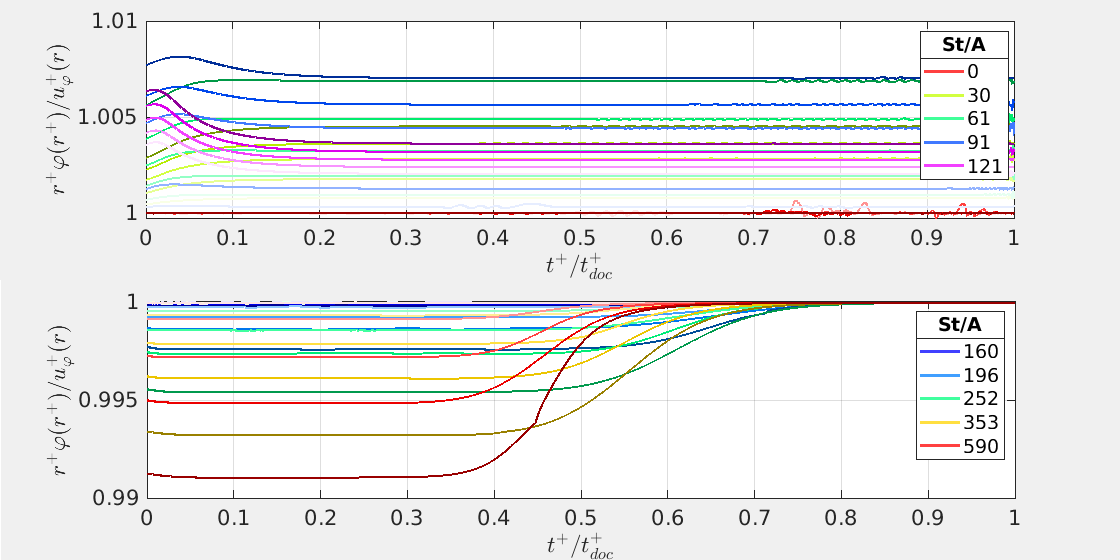
\includegraphics[width=30pc]{gfx/both_docking_ang_vel.png}
\caption{Angular velocity of a particle while docking at the axis (top) and in-orbit (bottom). X-axis is scaled separately for each trajectory by a docking time. On Y-axis, angular velocity is scaled by the fluid angular velocity at particle position. Line color corresponds to $St/A$ value, line color intensity to different $St$ and $A$ representations.}
\label{fig:ch3_450}
\end{figure*}

Unfortunately the attempt to simplify the equation of motion by assuming that particle angular velocity is equal to the fluid velocity at particle position leads to a contradiction - such an assumption could be made only in the linear vortex model. Even then the first of Eq.\ref{ch3:eq16} is a case of a Chini equation and in general it is not possible to solve it analytically. In-orbit docking radial velocity resembles a gaussian function and the radial position the error function (see Fig.\ref{fig:ch3_43}, but the tests proved they are not.\\
Now lets look closer at the axis docking process. Figures \ref{fig:ch3_42} and \ref{fig:ch3_44} show that  the particle firstly move with radial velocity the same as fluid's velocity: $v^+_r(r_s-\sigma)$. Next the particle radial velocity decreases rapidly in time. When the time is scaled by docking time, $t^+/t^+_{doc}$, the rate of this decrease depends on $St/A$ parameter only. Angular velocity increases towards fluid velocity close to the axis, $v^+_{\varphi}(\sigma)/\sigma$, when particle is approching the axis.\\
\noindent The first glance at \ref{fig:ch3_42} and \ref{fig:ch3_44} leads to the observation that the radial motion (as for $r(t)$ and $\dot{r}(t)$) of the particle docking on the axis resembles exponential decay. Logarithmic plots show these clearly linear dependence in time except for small times ($t^+<<t^+_{doc}$). Therefore, a simplified model of this process is proposed below and an attempt is made to estimate axis docking timescale $\tau^+_{d1}$.\\
Lets assume that in the axis docking process we have:
\begin{equation}
r^+(t) \propto \exp \frac{-t^+}{\tau^+_{d1}}
\label{ch3:eq22}
\end{equation}
and that $\tau^+_{d1}=\tau^+_{d1}(St,A)$.
\begin{figure*}
\centering
\noindent 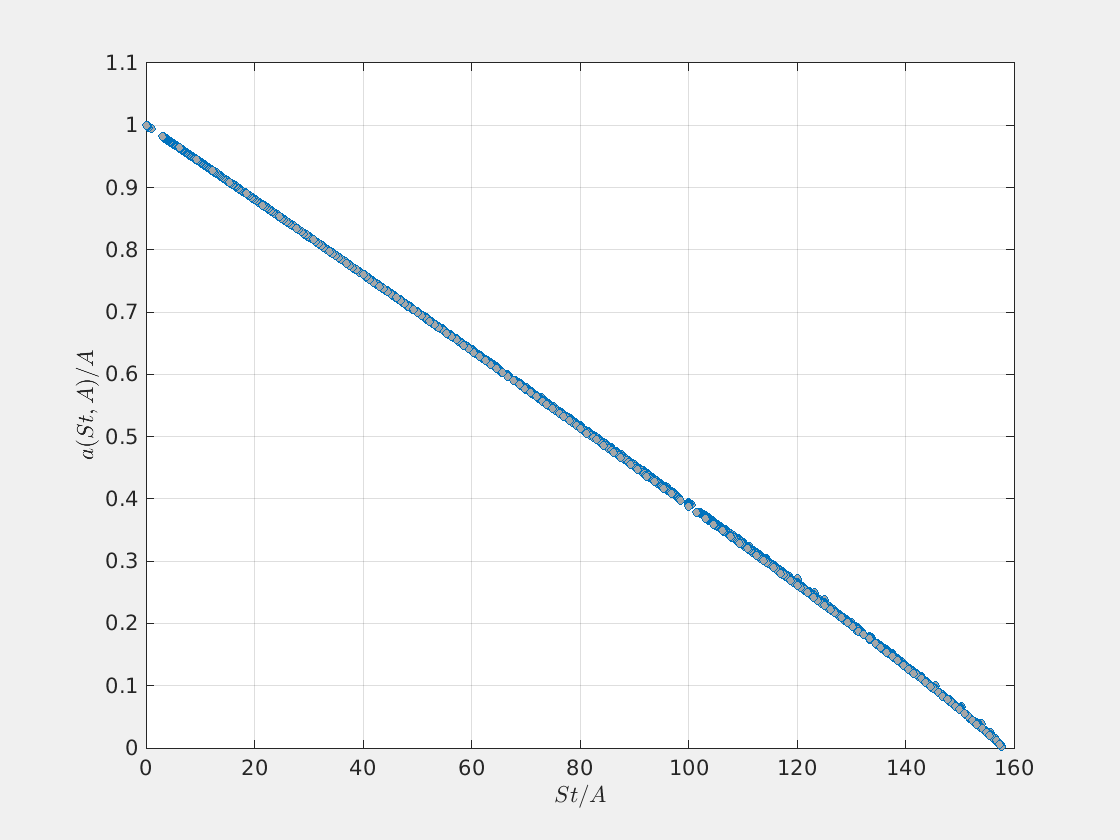
\includegraphics[width=30pc]{gfx/tau_d1_fit_vs_StA.png}
\caption{}
\label{fig:ch3_451}
\end{figure*}

I performed linear fit of the function $y=-a*x +b$ on the numerical trajectories for a range of $St$ and $A$, taking $y=\log r^+(t^+)$ and $x=t^+$. Figure \ref{fig:ch3_451} presents the directional coefficient fitted values in a way that reveals the relation with system parameters: on X-axis there is $St/A$ and on the Y-axis there is $a_{fit}/A$. It is clear that $\frac{a_{fit}}{A}$ depends only on $St/A$. In conclusion:

\begin{equation}
\frac{a_{fit}}{A} \approx \left(1-\frac{1}{16 \pi^2}\frac{St}{A}\right)
\label{ch3:eq22b}
\end{equation}

and further:
\begin{equation}
\tau^+_{d1}(St,A)\approx A^{-1}\left(1-(16 \pi^2)^{-1}\frac{St}{A}\right)^{-1}.
\label{ch3:eq22c}
\end{equation}
Dimensional axis docking timescale is then:
\begin{equation}
\tau_{d1} = \tau^+_{d1} \tau_f=2 \gamma^{-1} \left(1-(16 \pi^2)^{-1}\frac{St}{A}\right)^{-1}
\label{ch3:eq26}
\end{equation}
Estimated dimensional timescale $\tau_{d1}$ depends primarily on $\gamma^{-1}$. This is exactly the same as in the case of motion along vortex axis (see Eq.\ref{ch3:eq10}).\\

%When the time is scaled by docking time, $t^*=t^+/t^+_{doc}$, we expect as was stated before, that the exponential decay rate depends only on the parameter $St/A$:
%\begin{equation}
%r^+(t^*)\propto \exp\left(-h\left(St/A\right)t^*\right).
%\label{ch3:eq23}
%\end{equation}
%So in the end the docking time and timescale are related: $\tau^+_{d1}=t^+_{doc}(St,A))/h(St/A)$.
%
%
%
%%in-orbit
%After scaling the time by $t^+_{doc}$ it can be noticed that the docking process depends mainly monotonically on the parameter $St/A$. When its value decreases towards $16 \pi^2$ the docking time $t^+_{doc}$ tends to infinity.
%%%%
%Another obsevation is that when $St/A$ increases towards the critical value $16 \pi^2$, the docking time $t^+_{doc}$  tends to infinity.
%%%%%

Further the analysis of $t^+_{doc}$ for arbitrary parameter ranges was conducted. Figure \ref{fig:ch3_4} presents the results of $t^+_{doc}$ numerical calculation with respect to $St$ and $A$. The colorscale is logarithmic. Line that consists of local maxima respresents the $St=St_{cr}(A)$ boarder. For $St\approx St_{cr}(A)$ the forces working on the particle almost balance, so the docking time is very long. When approaching the critical value, it asymptotically goes to infinity.

\begin{figure*}
\centering
\noindent 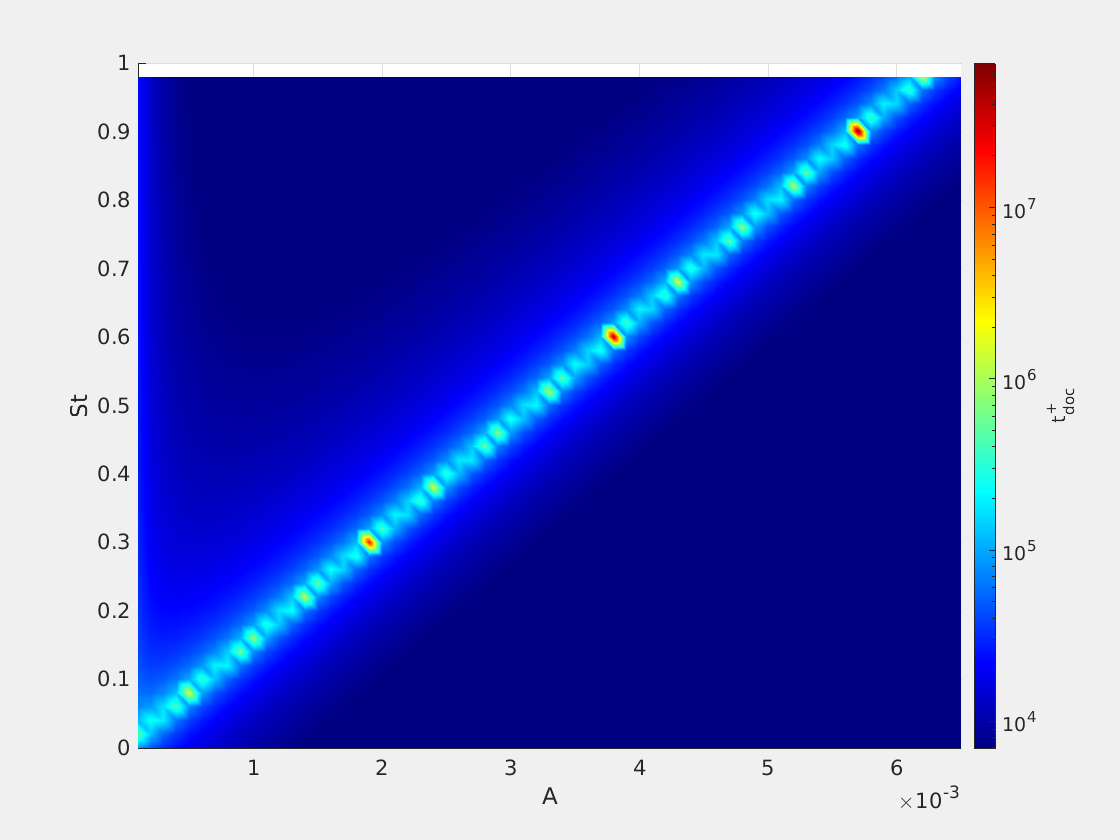
\includegraphics[width=30pc]{gfx/surf_logtdoc_vs_A_vs_St_full.png}
\caption{Docking time calculated numerically with respect to $St$ and $A$ for arbitrary variable ranges with $\sigma=10^{-5}$. Line of local maxima corresponds to $St=St_{cr}(A)$ and shows the stability boarder: particles to the left undergo in-orbit docking, particles to the right - axis docking.}
\label{fig:ch3_4}
\end{figure*}

Although the docking time is defined in a twofold way, it seems to have a physical meaning: the values are of a similar order, it goes towards on the both sides of the critical value.\\
Since $\sigma$ in theory is infinitesimally small but the numerical calculation demands finite value, the sensitivity analysis was conducted below for $\sigma=10^{-n}, \ n=1,2,3,4,5$. - do zrobienia jak starczy czasu.\\


\subsection{With gravity (inclined vortex)}
\noindent Nonparallel alignment of the gravity vector and vortex axis ($\theta \neq 0$) destroys the axial symmetry of the system and introduces the presence of other attractors, such as non-circular periodic orbit and multiple equilibrium points outside the axis.\\
 
For a nonzero $\theta$, every particle always has equilibrium points in 2D space. Position of these points in 2D space is determined by $S_v$ and $A$ and it can be uniquely determined by solving the equilibrium point equation:
\begin{equation}
 f_A(r^+) = S_v,
 \label{ch3:eq27}
\end{equation}
where function $f_A(r^+)$ is defined for each $A$:
\begin{equation}
f_A(r^+) = r^+ A \sqrt { 1 + \left( \frac{1-\exp \left(\frac{-r^{+ 2}}{2}\right)}{2\pi Ar^{+ 2}} \right)^2 }
 \label{ch3:eq28}
\end{equation}
and is called an equilibrium curve (see Fig.2 in \citet{Marcu1995}). Detailed analysis of this eqation's solutions is performed below.\\

\begin{table}
\small
\tabcolsep=0.2cm
\centering
\caption{Burgers vortex non-dimensional numbers}
\centering
\begin{tabular}{|l|c|}
\hline 
$A_{cr}$ & 0.02176 \\
\hline
$r_i$ & 2.1866\\
\hline
$S_{v i}$ & 0.0815\\
\hline
$r_s$ & 1.585201\\
\hline
$S_{v s}$ & 0.0718\\
\hline
\end{tabular}
\label{tab:ch3_2}
\end{table}

Equillibrium curves for a dozen of $A$ values are plotted in Fig. \ref{fig:ch3_6}. It is easy to find that $f_A(0)=0$ and $\lim_{r^+\to\infty} f_A(r^+)=\infty$. Moreover, there exists a critical value of nondimensional strain $A_{cr}$ for which bifurcation from one unique solution (for $A \geq A_{cr}$) to maximally three solutions (for $A<A_{cr}$) occurs. $A_{cr}$ corresponds to the equilibrium curve that has a horizontal slope at the inflection point. $A_{cr}$ value was estimated numerically (see the Table \ref{tab:ch3_2}). It is also easy to prove that the equillibrium curves asymptotically tend to the function $f_{A \rightarrow 0+}(r)=\left( 1-exp(-r^2/2)\right)/2\pi r$. This function, unlike equillibrium curves for $A \in (0,A_{cr})$ does not have a minimum.

\begin{figure*}
\centering
\noindent 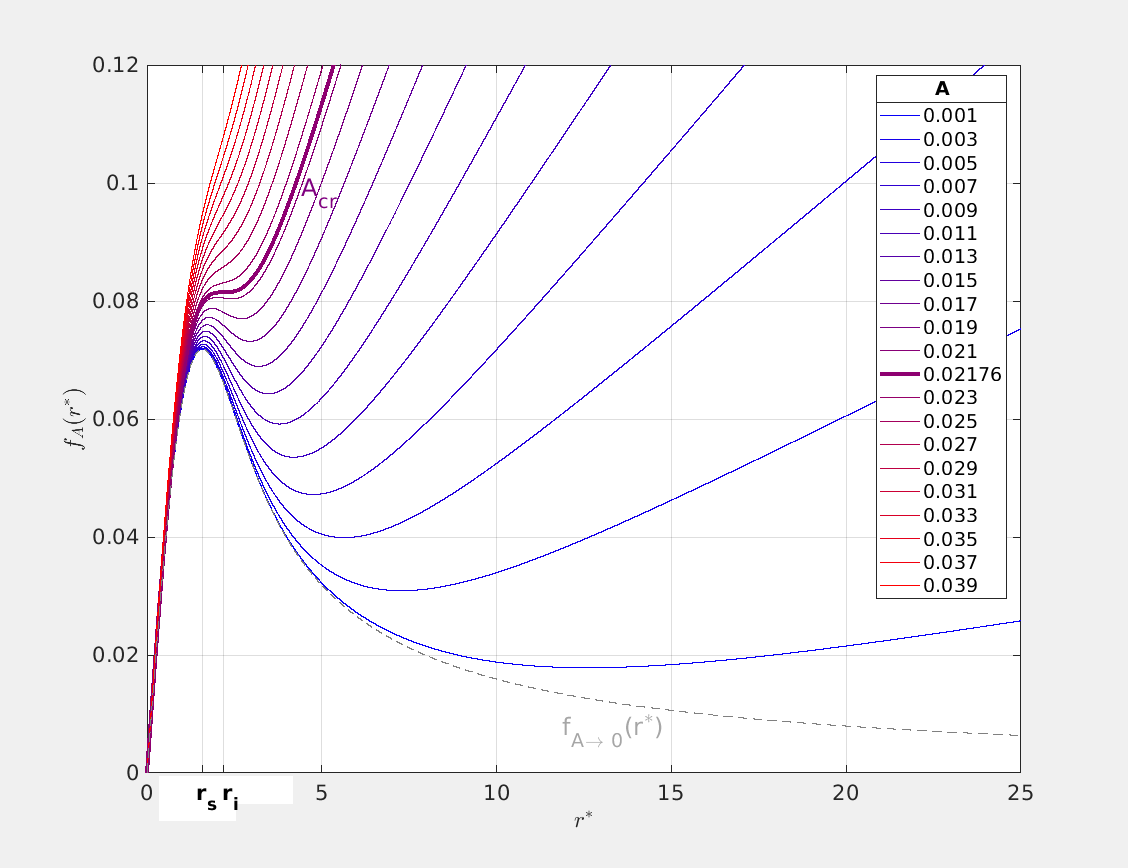
\includegraphics[width=30pc]{gfx/eq_curves.png}
\caption{Equillibrium curve plots for different $A$ values. $A_{cr}$, $r_s$, $r_i$ are defined in the text body. Gray dashed line shows an equillibrium curve which is an asymptotic limit of $A \rightarrow 0+$}
\label{fig:ch3_6}
\end{figure*}

For $A \geq A_{cr}$ the equilibrium curve is a monotonically increasing function of $r^+$ so there exists exactly one solution for every $S_v$ value.\\
For $A<A_{cr}$ the equilibrium curve always has one maximum at $r^+_{max}$ and one minimum at $r^+_{min}$. The inflection point of $A=A _{cr}$ equilibrium curve plot lies at $r_i$ and for $S_{v i}$ (numerical estimations in the Table \ref{tab:ch3_2}). It restricts values of $r^+_{max}$ from above and values of $r^+_{min}$ from below. Let's define:
\begin{align}
S_{v\ min}=f_A(r^+_{min}) \\
S_{v\ max}=f_A(r^+_{max})
\label{ch3:eq28b}
\end{align}
Consequently, for $S_v<S_{v\ min}$ and for $S_v>S_{v\ max}$, there is only one solution. For $S_v=S_{v\ min}$ and for $S_v=S_{v\ max}$, there are two solutions. For $S_{v\ min}<S_v<S_{v\ max}$, there are three solutions. All the conclusions are summarised in Table \ref{tab:ch3_2b}.

\begin{table}
\small
\tabcolsep=0.2cm
\caption{Existence and position of equilibrium points with respect to $A$ and $S_v$ parameters. $A_{cr}$, $r_s$, $r^+_{min}$, $S_{v\ min}$, $S_{v\ max}$ are defined in the text body.}
\centering
\begin{tabular}{|c|c|l|}
\hline
$A$ & $S_v$ & nr  of eq. points\\
\hline
$\geq A_{cr}$ & arbitrary & 1 \\
\hline
\multirow{3}{*}{$<A_{cr}$} & $<S_{v\ min}$ & 1 at $r^+_0 <r_s$ \\
\multirow{3}{*}{\ } & $[S_{v\ min},S_{v\ max}]$  & 2 or 3, I: $r^+_0\leq r^+_{max}<r_i$, II: $r^+_0 \in (r^+_{max},r^+_{min})$, III: $r^+_0>r^+_{min}$\\
\multirow{3}{*}{\ } & $>S_{v\ max}$  & 1 at $r^+_0>r^+_{min}>r_i$\\
\hline
\end{tabular}
\label{tab:ch3_2b}
\end{table}

Not only is the existence of the multiple solutions important but their stability as well. Let $r^+_0$ denote an arbitrary dimensionless solution of Eq. \ref{ch3:eq27}. The exact form of the stability condition of the solution $r^+_0$ is governed by the function $\phi(r^+_0)$ (defined in \citet{Marcu1995}). The condition can take two different forms depending on the sign of this function:
\begin{equation}
\phi(r^+_0)=\frac{1}{(2 \pi)^2} \left[\frac{1-\exp(-r^{+ 2}_0/2)}{r^{+ 2}_0} \right] \left[\frac{1-\exp(-r^{+ 2}_0/2)}{r^{+ 2}_0}-\exp(-r^{+ 2}_0/2) \right].
\label{ch3:eq29}
\end{equation}
Plots of $\phi(r^+_0)$ and its square root are shown in Fig.\ref{fig:ch3_7}.

\begin{figure*}
\centering
\noindent 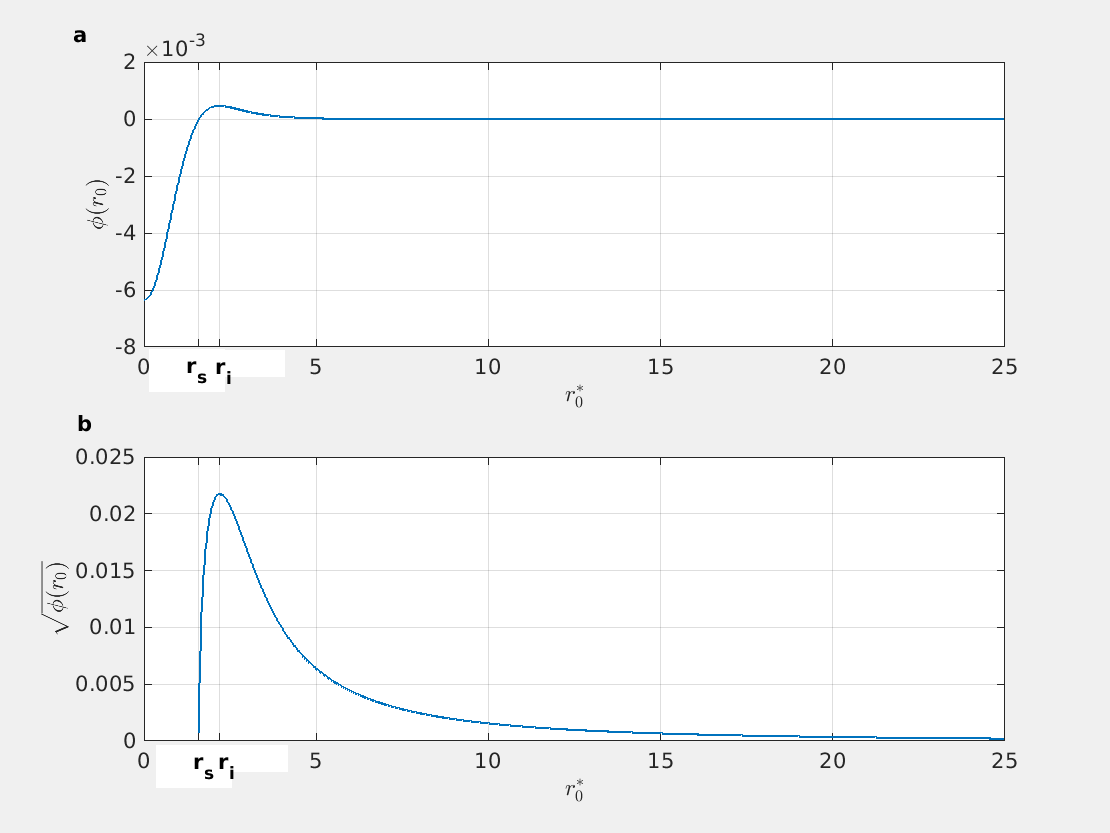
\includegraphics[width=30pc]{gfx/stability_functions.png}
\caption{Plot of the function $\phi(r^+_0)$ determining equillibrium point stability (a) and its square radius $\sqrt{\phi(r^+_0)}$ (b) with respect to equillibrium point radial position.}
\label{fig:ch3_7}
\end{figure*}

Function $\phi(r^+_0)$ has only one zero at $r_s$ (see Table \ref{tab:ch3_2}). For small radii, $r^+_0<r_s$, the equilibrium is a spiral/focus, and it is stable if:

\begin{equation}
St \leq \frac{A}{|{\phi(r^+_0)}|}.
\label{ch3:eq30}
\end{equation}

\noindent For greater radii, $r^+_0>r_s$, the equilibrium point is either a stable node or a saddle. The condition for stability depends explicitly only on $A$:
\begin{equation}
A \geq \sqrt{\phi(r^+_0)}.
\label{ch3:eq31}
\end{equation}
\\
Analysis of the equilibrium point stability conditions by \citet{Marcu1995} is expanded here with emphasis on the dependence on strain parameter $A$.  Because stability condition for larger radii $r^+_0 > r_s$ expressed by Eq.\ref{ch3:eq31} is independent of $St$, additional conclusions can be drawn. Numerical calculations lead to the result, that for every $A<A_{cr}$ there is:
\begin{equation}
\sqrt{\phi(r^+_{max}(A))}=\sqrt{\phi(r^+_{min}(A))}=A.
\label{ch3:eq32}
\end{equation}
In the range between maximum and minimum $r^+_0 \in (r^+_{max},r^+_{min})$ there is $\sqrt{\phi(r^+_0)} > \sqrt{\phi(r^+_{min}(A))}$, so the condition in Eq.\ref{ch3:eq31} is not satisfied and the points in this range are not stable. For $r^+_0 >r^+_{min}$ there is 
$\sqrt{\phi(r^+_0)} <\sqrt{\phi(r^+_{min}(A))}$, so the condition in Eq.\ref{ch3:eq31} is satisfied and the points in this range are stable.
In the case $A \geq A_{cr}$ the condition in Eq.\ref{ch3:eq31} is satisfied, because $A>\max_{r^+_0}\left( \sqrt{\varphi(r^+_0)}\right)=A_{cr}$. The unique solution is a stable node. These results are summarised in Table \ref{tab:ch3_3}.

\begin{table}
\small
\tabcolsep=0.2cm
\caption{Stability conditions of particle equilibrium points present in the Burgers vortex with respect to vortex strain parameter $A$ and dimensionless radial position $r^+$. $A_{cr}$, $\varphi(r^+)$, $r_s$, $r_i$, $r^+_{min}$ and $r^+_{max}$ are defined in the text body.}
\centering
\begin{tabular}{|l|c|c|c|c|}
\hline 
 & $ \leq r_s$ & $(r_s,r^+_{max})$ & $[r^+_{max}, r^+_{min})$ & $\geq r^+_{min}$ \\
\hline
$A < A_{cr}$ & \multirow{2}{*}{focus, unstable if $St>A/|\phi(r^+_0)|$} & stable node & saddle & stable node\\
\cline{3-5}
$A \geq A_{cr}$ &  \multirow{2}{*}{\ } & \multicolumn{3}{|c|}{stable node}\\
\hline
\end{tabular}
\label{tab:ch3_3}
\end{table}
 
The stability properties can be analysed with $S_v$ as a leading parameter too, in contrast to equilibrium curve viewpoint. Figure \ref{fig:ch3_8} presents equilibrium point $r^+_0$ plots versus $A$. Line colors refer to various $S_v$ parameters. Continuous line represents stable point, dashed - unstable. Three colored regions in the background mark three stability domains: light gray corresponds to condition in Eq.\ref{ch3:eq31} satisfied (a stable node), light green to the same condition not satisfied (a saddle), light red points to the focus region $r^+_0<r_s$. Stability of the focus is governed by Eq.\ref{ch3:eq30}, so $St$ must be considered as well. An example of stability properties in the region $r^+_0<r_s$ is shown by the cross signs - they represent the example of unstable foci for $St=0.5$. $r_s$, $r_i$ and $A_{cr}$ are marked on the axes for reference.

\begin{figure*}
\centering
\noindent 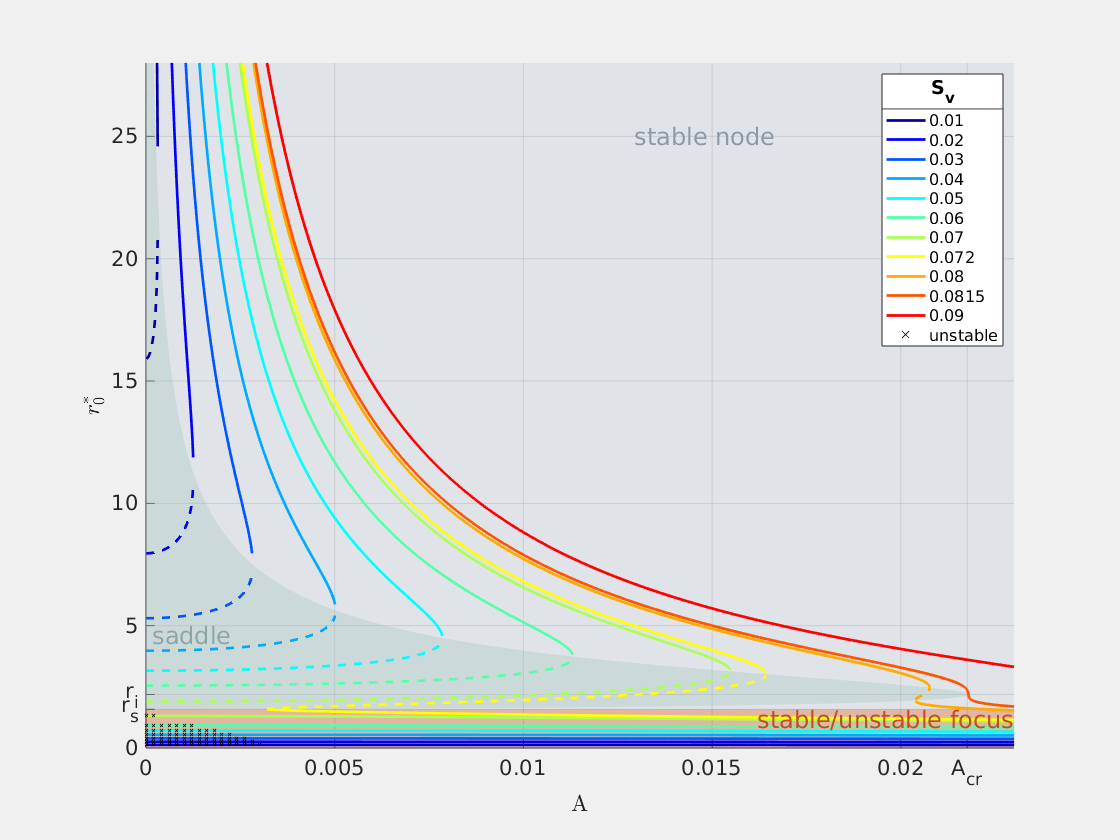
\includegraphics[width=30pc]{gfx/r0_vs_A_plus_stability.png}
\caption{Equilibrium point $r^+_0$ position versus $A$. Line colors refer to various $S_v$ parameters, continous line - to stable point, dashed line - to unstable. The colored regions in the background mark various stability subdomains: light gray - a stable node, light green - a saddle, light red - a focus. Crosses show example of unstable focii in the light red region for the case of $St=0.5$.}
\label{fig:ch3_8}
\end{figure*}

In Fig. \ref{fig:ch3_8}, the following conclusions about stability can be drawn.  For $S_v<S_{v s}$ there is at least one focus near the axis, at $r^+_0<r_s$, stable or unstable. When $A \geq A_{cr}$ it is unique, when $A<A_{cr}$ it can be accompied by a saddle and a stable node or a stable node itself. For $S_v \in (S_{v s},S_{v i})$ and when $A<A_{cr}$ there is at least the stable node far from the axis. In addition there can be the saddle and the stable node near the axis, the saddle and the focus or the focus itself. When $A \geq A_{cr}$ there is only one point near the axis and it is either a focus or a stable node. For $S_{v i}$ there is bifurcation from three possible solutions to just one. When $A<A_{cr}$ the one is a unique stable node far from the axis, when $A \geq A_{cr}$ it is a unique stable node at arbitrary position or a focus near the axis.\\

\begin{figure*}
\centering
\noindent 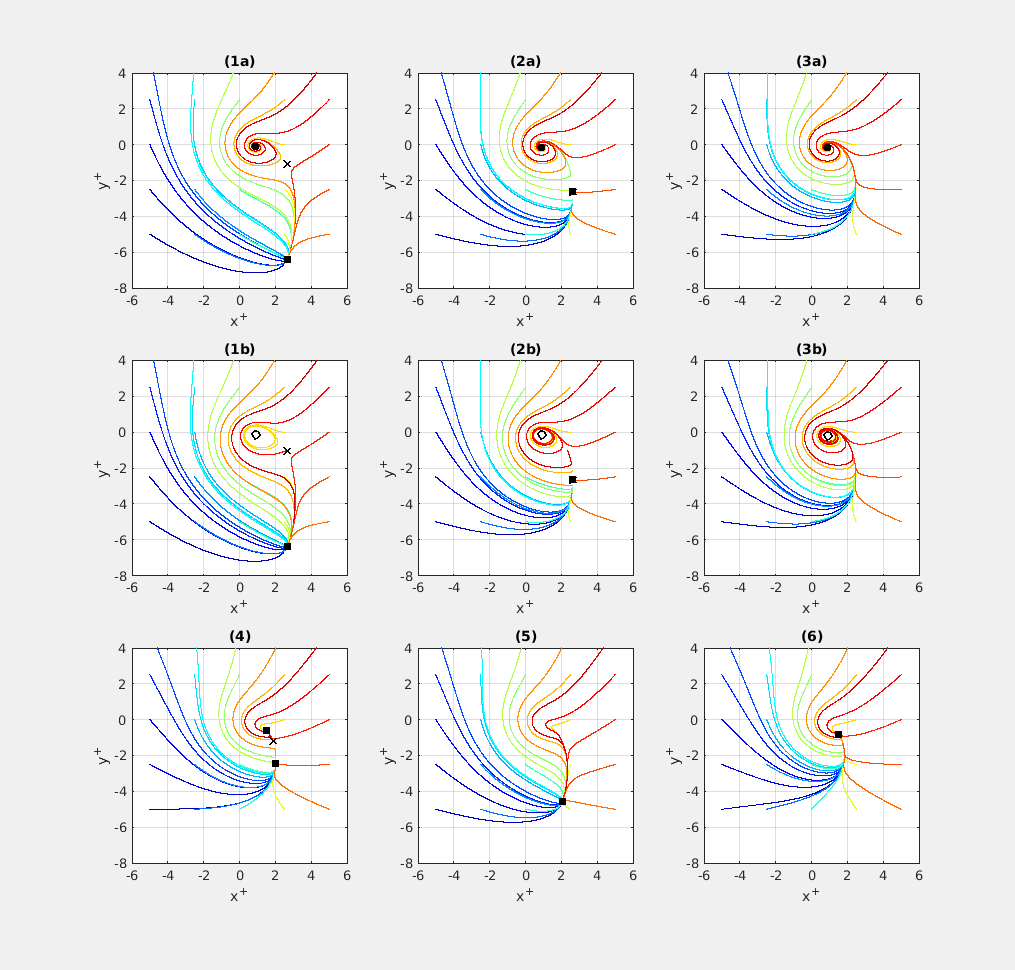
\includegraphics[width=30pc]{gfx/scenarios_9p_T500_D5_N5.png}
\caption{Particle trajectory plots for various sets of $(A,Sv,St)$ parameters. In each figure 25 particles are initialised at regular grid with zero velocity. Line colors vary in order to improve clarity. Scattered points represent equilibrium points position, their shape refer to their dynamical type: $\times$ - a saddle, $\circ$ - a focus (filled means stable), $\square$ - stable node. "a" and "b" types present the same $(A,Sv)$ sets, but with different $St$ determining stability of the focus ("a" - stable, "b" - unstable).}
\label{fig:ch3_9}
\end{figure*}

The combination of multiple point existence conditions with stability conditions creates a variety of single particle motion scenarios. Some of them were shown in Fig.4-9 in \citet{Marcu1995}. Fig. \ref{fig:ch3_9} here illustrates all nine of these combinations, by showing trajectory plots of particles initially positioned on the chosen grid with zero velocity. Trajectories were calculated numerically for representative sets of parameters. Different line colors are only intended to improve the plot clarity. Singular markers indicate the position of the equilibrium points, while their shape - their dynamic character. Tab.\ref{tab:ch3_4} summarises the analysis by showing $A$ and $Sv$ parameter ranges with relevant scenarios, as pictured in Fig. \ref{fig:ch3_9}. These scenarios are of particular interest in the context of void phenomenon explanation, especially the cases with limit cycle. This special solution and its properties are adressed next.

\begin{table}
\small
\tabcolsep=0.2cm
\caption{Single particle motion scenarios with respect to $A$ and $S_v$ parameters. Numbers refer to Fig.\ref{fig:ch3_9}}.
\centering
\begin{tabular}{|c|c|c|}
\hline 
 & $A < A_{cr}$ & $A \geq A_{cr}$\\
\hline
$S_v<S_{v s}$ &(1) (2) (3) & (3)\\
\hline
$[S_{v s},S_{v i}]$ & (1) (2) (4) (5)& (3) (6)\\
\hline
$S_v>S_{v i}$ & (5) & (3) (5) (6)\\
\hline
\end{tabular}
\label{tab:ch3_4}
\end{table}

Finding limit cycles in general is a very difficult problem, although there are important in many scientific applications. Numerical simulations show, that as $St/A-|\phi(r^+_0)|^{-1}$ passes through zero, Hopf bifurcation occures. It means that if the focus near the axis is unstable according to \ref{ch3:eq30}, then it is accompanied by a stable limic cycle. The limit cycle cannot be calculated analytically or approximately. However the condition in Eq.\ref{ch3:eq30} for unstable focus can be approximated. The assumption needed is that $r^\ast \leq r^\ast_s$. Firstly it allows to expand the relation for equillibrium point position as in Eq. \ref{eq27} in the vicinity of $r^{\ast}=0$. The other assumption is that in this vicinity the dependence on $A$ is weak (see Fig.2 in \citet{Marcu_95}).
\begin{equation}
\left(\frac{Sv}{A}\right)^2=r^{\ast 2} \left[1+ \left( \frac{1-\exp \left(-r^{\ast 2}/2\right)}{2\pi Ar^{\ast 2}} \right)^2 \right]=r^{\ast 2}+\frac{(1-\exp \left(-r^{\ast 2}/2\right))^2}{(2\pi A r^{\ast})^2}\simeq r^{\ast 2}+\frac{1}{4 \pi^2 A^2} \frac{r^{\ast 2}}{4}=r^{\ast 2}\left( 1+(4 \pi A)^{-2}\right),
\label{ch3:eq34}
\end{equation}
so in the end:
\begin{equation}
r^{\ast}_0\simeq 4 \pi Sv \left(1+(4\pi A)^2\right)^{-\frac{1}{2}}.
\label{eq11}
\end{equation}
It is equivalent to approximating vortex angular motion by rigid body rotation $u^+_{\varphi}=r^+/4\pi$.\\
Secondly, the function $\phi(r^\ast_0)$ is approximated as follows:
\begin{equation}
\phi(r^\ast_0)\simeq-(16 \pi^2)^{-1}(1-r^\ast_0).
\label{ch3:eq35}
\end{equation}

At $r^{\ast}=0$ stability condition takes the same form as for the case without gravity.\\
\noindent The (un)stability condition, which is to the best knowledge equivalent to existence of a limit cycle, after algebraic transformations comes down to the requirement that the strain parameter is small enough $A < A_{max}$ and consequently circulation large enough $\Gamma > \Gamma_{min}$, where the $A_{max}$ value is estimated as follows:
\begin{align}
P \equiv 1+\nu^{-1}g^2\tau_p^3\sin^2\theta-2^{-1}\tau_p\gamma,\\
A_{max}=\left[2^{-1} (4\pi)^{-2} P  ((1+2\frac{\tau_p\gamma}{P^2})^{\frac{1}{2}} - 1 )\right]^{\frac{1}{2}}.
\label{ch3:eq36}
\end{align}

\noindent The maximal strain parameter $A_{max}$ (minimal circulation $\Gamma_{min}$) increases (decreases) weakly with $P$. However the direct link to system parameters is intricate. Fig.\ref{fig:ch3_10} presents its value vs. particle radius and vortex core size for an arbitrary alignment angle.
\begin{figure*}
\centering
\noindent 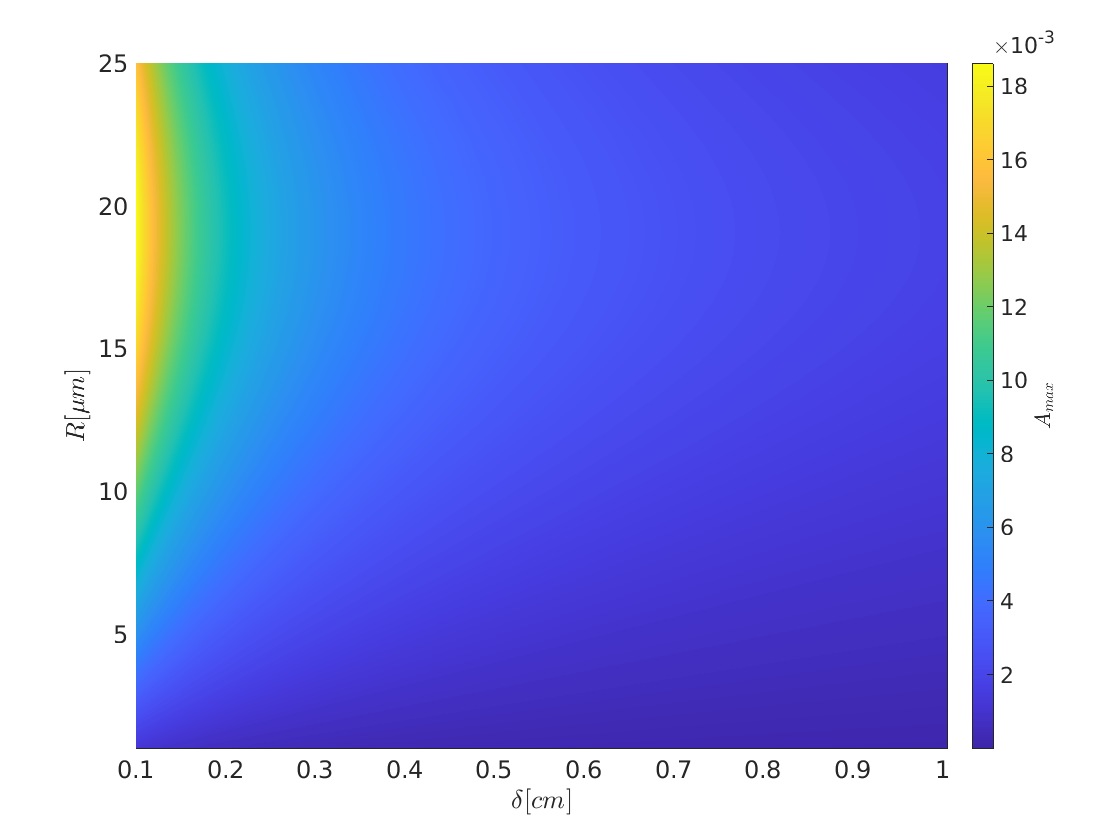
\includegraphics[width=30pc]{gfx/Amax_vs_delta_vs_R.png}
\caption{Maximal strain parameter $A_{max}$ with respect to vortex core size $\delta$ and particle radius $R$, for an arbitrary alignment angle $\theta=\pi/4$.}
\label{fig:ch3_10}
\end{figure*}
Figure \ref{fig:ch3_11} presents the same relation in a slightly different form. There are just a few $\delta$ values explored. Each coloured band represents $A_{max}$ range obtained  for a bundle of alignment angles $\theta \in (0,\pi/2)$. The dependence between $A_{max}$ and $R$ is clearly linear when $\theta=0$. In fact in such a case it agrees with the relation shown in \ref{ch3:eq19a}.

\begin{figure*}
\centering
\noindent 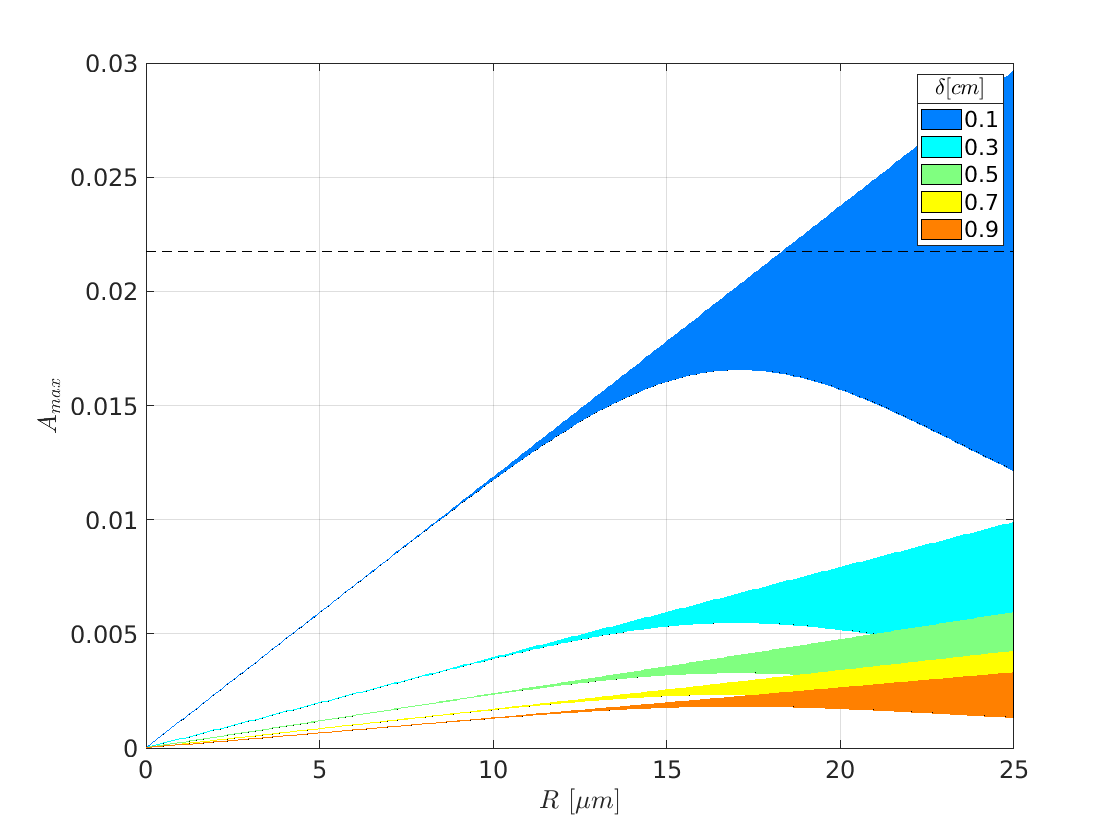
\includegraphics[width=30pc]{gfx/Amax_vs_R.png}
\caption{Maximal strain parameter $A_{max}$ with respect to  particle radius $R$ for a few vortex core sizes $\delta$, drawn for a bundle of alignment angles. $A_{cr}$  value is shown with a dashed line.}
\label{fig:ch3_11}
\end{figure*}


Finally we can formulate the general conclusion that increasing vortex core size $\delta$ or decreasing particle size (when $\theta$ is not large) causes the decrease in $A_{max}$ (equivalent to increase in minimal circulation $\Gamma_{min}$).\\
...\\
Dodac cos tutaj o tej publikacji Sapsin And Haler 2010 o przyciaganiu czastek inercyjnych przez powolne rozmaitosci. - jesli starczy czasu.

\section{Time scales of single particle motion}

\begin{table}
\small
\tabcolsep=0.2cm
\caption{Summary of single particle motion timescales}.
\centering
\begin{tabular}{|l|}
\hline 
$\tau_z\approx 2\gamma^{-1}$\\
\hline 
$\tau_{ex}(Z^\ast,z_0^\ast; \tau_z)\approx \tau_z \log\left(L(Z^\ast,z_0^\ast)\right)$\\
\hline 
$\tau_{orb}=\sqrt{2 \tau_p \gamma^{-1}}$\\
\hline
$\tau_{d1} =2 \gamma^{-1} \left(1-\frac{St}{(4\pi)^{2} A}\right)^{-1}$\\
\hline
\end{tabular}
\label{tab:ch3_5}
\end{table}

Approximate relations of a few timescales for single particle motion in Burgers vortex were found: exit time $\tau_{ex}$, connected to timescale of motion along the axis $\tau_z$, no-gravity orbit rotation timescale $\tau_{orb}$ and no-gravity axis docking timescale $\tau_{d1}$. For ease of reference, these approximations are summarised in Table \ref{tab:ch3_5}. Several conclusions about three dimensional particle motion can be drawn from the comparison of the separately derived time scales:
\begin{enumerate}
\item $\tau_z$ is approx. independent of particle radius $R$ and vortex strain $A$.
\item $\tau_{orb}<<\tau_z$, so as long as the logarithmic part in Eq.\ref{ch3:eq14} is not significantly smaller than 1, the particle starting far from vortex "lids' is able to swirl around the vortex axis for significant amount of time before being expelled by motion along vortex axis.
\item The relation between axis docking timescale and motion along the axis timescale depends primarily on $St/A$ parameter:
\begin{equation}
\frac{\tau_z}{\tau_{d1}} = 1-\frac{St}{(4 \pi)^2 A}.
\label{ch3:eq33}
\end{equation}
If $St/A \approx 0$, then $\tau_z \approx \tau_{d1}$. Increasing $St/A$ causes $\tau_z$ to be smaller then $\tau_{d1}$. It means that in general, particles are expelled from the vortex  through its lids faster then approach the vortex axis in docking process. The difference is larger the larger $St/A$ is. The exact relation between process times depend on the initial conditions of particle motion as well.
\end{enumerate} 

\section{Summary}
The subject of this chapter was the motion of a single finite-size particle subjected to viscosity and gravity forces only, in a steady fluid motion modelled by a Burgers vortex with stretching. This analysis bridged the gaps and deepened the knowledge on the subject presented in the paper of \citet{Marcu1995} and by setting a relation to conditions expected in atmospheric clouds.
Generally it proves the hypothesis that the nature of 3D cloud droplet motion in such a simplified system is complex and very much dependent on the parameters of the model, which are here vortex stretching, strain, alignment angle and particle size. It cannot be easily reduced or approximated. Particle motion in 2D is governed by orbit attraction/repulsion, which are foci, nodes, circular periodic orbit and/or limit cycle. How much the presence of these orbits determines the total motion of a particle in 3D is primarily influenced by the ratio of time scales of motion in 2D and along the axis. This ratio can be explicitly specified only in selected cases of motion. The intuition suggests that when it comes to multi-particle, polydisperse system, these results demonstrate a great potential in particle segregation, clustering and relative velocity influence.

\end{document}